% Seminarul 9: Modele ARCH și GARCH
% Statistica piețelor financiare -- Program de licență, Academia de Studii Economice din București
% GENERAT de latex/build_seminar9.py -- modificați generatorul, nu acest fișier.
% Implicit versiunea pentru studenți; versiunea profesorului este wrapper-ul *_solutions.tex.
\makeatletter\@ifundefined{ifsolutions}{\expandafter\newif\csname ifsolutions\endcsname}{}\makeatother

\newcommand{\coursename}{Statistica piețelor financiare}
\def\sfmlang{ro}
% Preambul comun SFM -- Statistica piețelor financiare / Statistics of Financial Markets (Beamer, 16:9)
% Același design ca MFM. Înainte de % Preambul comun SFM -- Statistica piețelor financiare / Statistics of Financial Markets (Beamer, 16:9)
% Același design ca MFM. Înainte de % Preambul comun SFM -- Statistica piețelor financiare / Statistics of Financial Markets (Beamer, 16:9)
% Același design ca MFM. Înainte de \input{../../latex/preamble} se definește
%   \newcommand{\coursename}{Statistics of Financial Markets}      (EN)
%   \newcommand{\coursename}{Statistica piețelor financiare}       (RO)  și  \def\sfmlang{ro}
% Fișierele .tex se află în EN/Courses, EN/Seminars, RO/Cursuri, RO/Seminarii (două niveluri sub rădăcină).
% Deck-urile sînt generate de latex/build_chapterN.py / build_seminarN.py (vezi latex/sfm_build.py).

\documentclass[9pt, aspectratio=169, t]{beamer}
\providecommand{\coursename}{Statistics of Financial Markets}

% Ensure content fits on slides
\setbeamersize{text margin left=8mm, text margin right=8mm}

%=============================================================================
% THEME AND STYLE CONFIGURATION
%=============================================================================
\usetheme{default}
% Using default theme for clean header/footer control

% Color Palette (matching Redispatch PDF)
\definecolor{MainBlue}{RGB}{26, 58, 110}
\definecolor{AccentBlue}{RGB}{26, 58, 110}
\definecolor{IDAred}{RGB}{205, 0, 0}
\definecolor{DarkGray}{RGB}{51, 51, 51}
\definecolor{MediumGray}{RGB}{128, 128, 128}
\definecolor{LightGray}{RGB}{248, 248, 248}
\definecolor{VeryLightGray}{RGB}{235, 235, 235}
\definecolor{KeynoteGray}{RGB}{218, 218, 218}
\definecolor{SectionGray}{RGB}{120, 120, 120}
\definecolor{FooterGray}{RGB}{100, 100, 100}
\definecolor{Crimson}{RGB}{220, 53, 69}
\definecolor{Forest}{RGB}{46, 125, 50}
\definecolor{Amber}{RGB}{181, 133, 63}
\definecolor{Orange}{RGB}{230, 126, 34}
\definecolor{Purple}{RGB}{142, 68, 173}

% Gradient background (exact Keynote 315° gradient: white to RGB 218,218,218)
\setbeamertemplate{background}{%
    \begin{tikzpicture}[remember picture, overlay]
        \shade[shading=axis, shading angle=315,
        top color=white, bottom color=KeynoteGray]
        (current page.south west) rectangle (current page.north east);
    \end{tikzpicture}%
}
% Fallback solid color for compatibility
\setbeamercolor{background canvas}{bg=}

\setbeamercolor{palette primary}{bg=MainBlue, fg=white}
\setbeamercolor{palette secondary}{bg=MainBlue!85, fg=white}
\setbeamercolor{palette tertiary}{bg=MainBlue!70, fg=white}
\setbeamercolor{structure}{fg=MainBlue}
\setbeamercolor{title}{fg=IDAred}
\setbeamercolor{frametitle}{fg=IDAred, bg=}
\setbeamercolor{block title}{bg=MainBlue, fg=white}
\setbeamercolor{block body}{bg=VeryLightGray, fg=DarkGray}
\setbeamercolor{block title alerted}{bg=Crimson, fg=white}
\setbeamercolor{block body alerted}{bg=Crimson!8, fg=DarkGray}
\setbeamercolor{block title example}{bg=Forest, fg=white}
\setbeamercolor{block body example}{bg=Forest!8, fg=DarkGray}
\setbeamercolor{item}{fg=MainBlue}

% Footer colors (override Madrid theme blue)
\setbeamercolor{author in head/foot}{fg=FooterGray, bg=}
\setbeamercolor{title in head/foot}{fg=FooterGray, bg=}
\setbeamercolor{date in head/foot}{fg=FooterGray, bg=}
\setbeamercolor{section in head/foot}{fg=FooterGray, bg=}
\setbeamercolor{subsection in head/foot}{fg=FooterGray, bg=}

% Bullet styles (apply everywhere including blocks)
\setbeamertemplate{itemize item}{\color{MainBlue}$\boxdot$}
\setbeamertemplate{itemize subitem}{\color{MainBlue}$\blacktriangleright$}
\setbeamertemplate{itemize subsubitem}{\color{MainBlue}\tiny$\bullet$}
\setbeamertemplate{itemize/enumerate body begin}{\normalsize}
\setbeamertemplate{itemize/enumerate subbody begin}{\normalsize}

% Item spacing - compact style
\setlength{\leftmargini}{10pt}       % Level 1: minimal indent
\setlength{\leftmarginii}{10pt}      % Level 2: minimal additional indent
% Compact list spacing (zero extra space before/after lists in blocks)
\makeatletter
\def\@listi{\leftmargin\leftmargini \topsep 0pt \parsep 0pt \itemsep 0pt}
\def\@listii{\leftmargin\leftmarginii \topsep 0pt \parsep 0pt \itemsep 0pt}
\makeatother

\setbeamertemplate{navigation symbols}{}

%=============================================================================
% CUSTOM HEADLINE
%=============================================================================
\setbeamertemplate{headline}{%
    \vskip10pt%
    \hbox to \paperwidth{%
        \hskip0.5cm%
        {\small\color{FooterGray}\renewcommand{\hyperlink}[2]{##2}\insertsectionhead}%
        \hfill%
        \textcolor{FooterGray}{\small\insertframenumber}%
        \hskip0.5cm%
    }%
    \vskip4pt%
    {\color{FooterGray}\hrule height 0.4pt}%
}

%=============================================================================
% CUSTOM FOOTER
%=============================================================================
\usepackage{fontawesome5}

\setbeamertemplate{footline}{%
    {\color{FooterGray}\hrule height 0.4pt}%
    \vskip4pt%
    \hbox to \paperwidth{%
        \hskip0.5cm%
        \textcolor{FooterGray}{\small\coursename}%
        \hfill%
        \raisebox{-0.1em}{%
            \begin{tikzpicture}[x=0.08em, y=0.08em, line width=0.4pt]
                \draw[FooterGray] (0,3) -- (1,4) -- (2,3.5) -- (3,5) -- (4,4) -- (5,6) -- (6,5.5) -- (7,4) -- (8,5) -- (9,7) -- (10,6) -- (11,5) -- (12,6.5) -- (13,8) -- (14,7) -- (15,6) -- (16,7.5) -- (17,9) -- (18,8) -- (19,7) -- (20,8.5) -- (21,10) -- (22,9) -- (23,8) -- (24,9.5);
            \end{tikzpicture}%
        }%
        \hskip0.5cm%
    }%
    \vskip6pt%
}

%=============================================================================
% PACKAGES
%=============================================================================
\usepackage[utf8]{inputenc}
\DeclareUnicodeCharacter{03B1}{\ensuremath{\alpha}}
\usepackage[T1]{fontenc}
\usepackage{amsmath, amssymb, amsthm}
\usepackage{mathtools}
\usepackage{bm}
\usepackage{tikz}
\usetikzlibrary{arrows.meta, positioning, shapes, calc, decorations.pathreplacing, shadings}
\usepackage{booktabs}
\usepackage{multirow}
\usepackage{array}
\usepackage{graphicx}
\usepackage{hyperref}
\usepackage{colortbl}
\usepackage{listings}
\lstset{language=Python, basicstyle=\ttfamily\scriptsize, keywordstyle=\color{MainBlue}\bfseries,
  commentstyle=\color{Forest}, stringstyle=\color{Crimson}, breaklines=true,
  frame=none, backgroundcolor=\color{VeryLightGray}, xleftmargin=2mm}
\hypersetup{colorlinks=true, linkcolor=MainBlue, urlcolor=MainBlue}
\graphicspath{{../../logos/}{../../charts/}{../../photos/}}
\usepackage{xcolor}
\hfuzz=2pt  % Suppress tiny overfull warnings (<2pt)
\vfuzz=2pt  % Suppress tiny vertical overfull warnings (<2pt)

%=============================================================================
% QUANTLET COMMANDS
%   \quantlet{<displayed name>}{<url>}       (generic, compatible with the older SFM decks)
%   \sfmquantlet{Ch_05}{SFM_ch5_garch}       -> https://github.com/danpele/SFM/tree/main/Quantlets/Ch_05/SFM_ch5_garch
%   \qlurl{<folder>} is defined per chapter by the generator (Quantlets/Ch_NN/<folder>)
%=============================================================================
\newcommand{\sfmrepo}{https://github.com/danpele/SFM}
\newcommand{\sfmqlbase}{https://github.com/danpele/SFM/tree/main/Quantlets}
\newcommand{\quantlet}[2]{%
    \hfill\href{#2}{%
        \raisebox{-0.15em}{
\includegraphics[height=0.7em]{ql_logo.png}}%
        \textcolor{MainBlue}{\tiny\ #1}%
    }%
}
\newcommand{\sfmquantlet}[2]{\quantlet{\detokenize{#2}}{\sfmqlbase/#1/#2}}

%=============================================================================
% NOTEBOOKS (Google Colab)
%   \colaburl{notebooks/EN/chapter5_seminar_notebook.ipynb} -> the Colab link of a file in the SFM repo
%   \nb: the chapter notebook (each seminar deck redefines it with \renewcommand)
%=============================================================================
\newcommand{\colaburl}[1]{https://colab.research.google.com/github/danpele/SFM/blob/main/#1}
\newcommand{\nb}{https://colab.research.google.com/github/danpele/SFM/tree/main/notebooks/EN}
\newcommand{\nbname}{notebooks/EN}

%=============================================================================
% SLIDE HELPERS (used by the generators; the same as in MFM)
%=============================================================================
% local font size for list bodies (the preamble forces \normalsize)
\newcommand{\itemsize}[1]{\setbeamertemplate{itemize/enumerate body begin}{#1}\setbeamertemplate{itemize/enumerate subbody begin}{#1}}
\newcommand{\intitle}[1]{{\hypersetup{urlcolor=white}#1}}   % white links inside coloured title bars
\newcommand{\imgcap}[1]{{\scriptsize #1}\\[0.5mm]}          % caption under a photo
\newcommand{\imgcredit}[2]{{\tiny\color{FooterGray}\href{#1}{#2}}}   % image credit: source URL, author/licence
\newcommand{\aiprompt}[1]{{\ttfamily\color{MainBlue}#1}}     % a prompt to an AI assistant

%=============================================================================
% SEMINARS: student version by default; the instructor wrapper *_solutions.tex sets \solutionstrue
%=============================================================================
\makeatletter\@ifundefined{ifsolutions}{\expandafter\newif\csname ifsolutions\endcsname}{}\makeatother
\newcommand{\solonly}[1]{\ifsolutions #1\fi}
\newcommand{\propsub}{\ifsolutions\else\framesubtitle{\ifdefined\sfmlang Rezolvarea se discută la seminar\else Solution discussed in class\fi}\fi}

%=============================================================================
% APPENDIX AND CHAPTER LINKS (latex/appendix_links.py writes the calls; it also re-declares these
% macros before \begin{document}, so the decks compile with or without this preamble block)
%=============================================================================
\providecommand{\sfmapplink}[3]{\hypertarget{#2}{}\hyperlink{#1}{\beamergotobutton{#3}}}
\providecommand{\sfmappback}[2]{\begin{tikzpicture}[remember picture,overlay]\node[anchor=south east] at ([xshift=-3mm,yshift=7mm]current page.south east){\hyperlink{#1}{\beamerreturnbutton{#2}}};\end{tikzpicture}}
\providecommand{\sfmchlink}[2]{\href{#1}{#2}}
\providecommand{\sfmchlinkt}[2]{\href{#1}{\usebeamercolor[fg]{frametitle}#2}}

%=============================================================================
% QUANTINAR COMMAND: link către un curs Quantinar (subiecte avansate)
%=============================================================================
\newcommand{\quantinar}[2]{%
    \href{#2}{%
        \raisebox{-0.15em}{
\includegraphics[height=0.8em]{qr_logo.png}}%
        \textcolor{MainBlue}{\scriptsize\ #1}%
    }%
}

%=============================================================================
% CUSTOM TITLE PAGE
%=============================================================================
\defbeamertemplate*{title page}{hybrid}[1][]
{
    \vspace{0.2cm}
    % Logos row - top header (with clickable links)
    \begin{center}
        \href{https://www.ase.ro}{
\includegraphics[height=1.0cm]{ase_logo.png}}\hspace{0.3cm}%
        \href{https://theida.net}{
\includegraphics[height=1.0cm]{ida_logo.png}}\hspace{0.3cm}%
        \href{https://blockchain-research-center.com}{
\includegraphics[height=1.0cm]{brc_logo.png}}\hspace{0.3cm}%
        \href{https://www.ai4efin.ase.ro}{
\includegraphics[height=1.0cm]{ai4efin_logo.png}}\hspace{0.3cm}%
        \href{https://ipe.ro/new}{
\includegraphics[height=1.0cm]{acad_logo.png}}\hspace{0.3cm}%
        \href{https://www.digital-finance-msca.com}{
\includegraphics[height=1.0cm]{msca_logo.png}}%
    \end{center}

    \vspace{0.6cm}

    % Main title with Q logos on sides (with clickable links)
    \begin{center}
        \begin{minipage}{0.1\textwidth}
            \centering
            \href{https://quantlet.com}{
\includegraphics[height=1.1cm]{ql_logo.png}}
        \end{minipage}%
        \begin{minipage}{0.78\textwidth}
            \centering
            {\LARGE\bfseries\usebeamercolor[fg]{title}\inserttitle}

            \vspace{0.3cm}

            {\usebeamerfont{subtitle}\usebeamercolor[fg]{title}\insertsubtitle}
        \end{minipage}%
        \begin{minipage}{0.1\textwidth}
            \centering
            \href{https://quantinar.com}{
\includegraphics[height=1.1cm]{qr_logo.png}}
        \end{minipage}
    \end{center}

    \vspace{0.6cm}

    % Authors (left aligned)
    \hspace{0.5cm}{\usebeamerfont{author}\insertauthor}

    \vspace{0.3cm}

    % Institute/Affiliations (left aligned)
    \hspace{0.5cm}\begin{minipage}[t]{0.9\textwidth}
        \raggedright\small\insertinstitute
    \end{minipage}
}

%=============================================================================
% THEOREM ENVIRONMENTS
%=============================================================================
\theoremstyle{definition}
\setbeamertemplate{theorems}[numbered]
\ifdefined\sfmlang
\newtheorem{defn}{Definiție}
\newtheorem{thm}{Teoremă}
\newtheorem{prop}{Propoziție}
\newtheorem{rmk}{Observație}
\else
\newtheorem{defn}{Definition}
\newtheorem{thm}{Theorem}
\newtheorem{prop}{Proposition}
\newtheorem{rmk}{Remark}
\fi

%=============================================================================
% CENTRED MINIPAGE (no extra vertical space)
%=============================================================================
\newenvironment{cminipage}[1]{%
    \par\noindent\hfill\begin{minipage}{#1}\ignorespaces
}{%
    \end{minipage}\hfill\null\par
}

%=============================================================================
% CUSTOM COMMANDS
%=============================================================================
\newcommand{\E}{\mathbb{E}}
\newcommand{\Var}{\text{Var}}
\newcommand{\Cov}{\text{Cov}}
\newcommand{\Corr}{\text{Corr}}
\newcommand{\R}{\mathbb{R}}
\newcommand{\N}{\mathbb{N}}
\newcommand{\Z}{\mathbb{Z}}
\newcommand{\B}{\mathbf{B}}
\newcommand{\imark}{\textcolor{MainBlue}{\textbullet}}
\newcommand{\RMSE}{\text{RMSE}}
\newcommand{\MAE}{\text{MAE}}
\newcommand{\MAPE}{\text{MAPE}}

 se definește
%   \newcommand{\coursename}{Statistics of Financial Markets}      (EN)
%   \newcommand{\coursename}{Statistica piețelor financiare}       (RO)  și  \def\sfmlang{ro}
% Fișierele .tex se află în EN/Courses, EN/Seminars, RO/Cursuri, RO/Seminarii (două niveluri sub rădăcină).
% Deck-urile sînt generate de latex/build_chapterN.py / build_seminarN.py (vezi latex/sfm_build.py).

\documentclass[9pt, aspectratio=169, t]{beamer}
\providecommand{\coursename}{Statistics of Financial Markets}

% Ensure content fits on slides
\setbeamersize{text margin left=8mm, text margin right=8mm}

%=============================================================================
% THEME AND STYLE CONFIGURATION
%=============================================================================
\usetheme{default}
% Using default theme for clean header/footer control

% Color Palette (matching Redispatch PDF)
\definecolor{MainBlue}{RGB}{26, 58, 110}
\definecolor{AccentBlue}{RGB}{26, 58, 110}
\definecolor{IDAred}{RGB}{205, 0, 0}
\definecolor{DarkGray}{RGB}{51, 51, 51}
\definecolor{MediumGray}{RGB}{128, 128, 128}
\definecolor{LightGray}{RGB}{248, 248, 248}
\definecolor{VeryLightGray}{RGB}{235, 235, 235}
\definecolor{KeynoteGray}{RGB}{218, 218, 218}
\definecolor{SectionGray}{RGB}{120, 120, 120}
\definecolor{FooterGray}{RGB}{100, 100, 100}
\definecolor{Crimson}{RGB}{220, 53, 69}
\definecolor{Forest}{RGB}{46, 125, 50}
\definecolor{Amber}{RGB}{181, 133, 63}
\definecolor{Orange}{RGB}{230, 126, 34}
\definecolor{Purple}{RGB}{142, 68, 173}

% Gradient background (exact Keynote 315° gradient: white to RGB 218,218,218)
\setbeamertemplate{background}{%
    \begin{tikzpicture}[remember picture, overlay]
        \shade[shading=axis, shading angle=315,
        top color=white, bottom color=KeynoteGray]
        (current page.south west) rectangle (current page.north east);
    \end{tikzpicture}%
}
% Fallback solid color for compatibility
\setbeamercolor{background canvas}{bg=}

\setbeamercolor{palette primary}{bg=MainBlue, fg=white}
\setbeamercolor{palette secondary}{bg=MainBlue!85, fg=white}
\setbeamercolor{palette tertiary}{bg=MainBlue!70, fg=white}
\setbeamercolor{structure}{fg=MainBlue}
\setbeamercolor{title}{fg=IDAred}
\setbeamercolor{frametitle}{fg=IDAred, bg=}
\setbeamercolor{block title}{bg=MainBlue, fg=white}
\setbeamercolor{block body}{bg=VeryLightGray, fg=DarkGray}
\setbeamercolor{block title alerted}{bg=Crimson, fg=white}
\setbeamercolor{block body alerted}{bg=Crimson!8, fg=DarkGray}
\setbeamercolor{block title example}{bg=Forest, fg=white}
\setbeamercolor{block body example}{bg=Forest!8, fg=DarkGray}
\setbeamercolor{item}{fg=MainBlue}

% Footer colors (override Madrid theme blue)
\setbeamercolor{author in head/foot}{fg=FooterGray, bg=}
\setbeamercolor{title in head/foot}{fg=FooterGray, bg=}
\setbeamercolor{date in head/foot}{fg=FooterGray, bg=}
\setbeamercolor{section in head/foot}{fg=FooterGray, bg=}
\setbeamercolor{subsection in head/foot}{fg=FooterGray, bg=}

% Bullet styles (apply everywhere including blocks)
\setbeamertemplate{itemize item}{\color{MainBlue}$\boxdot$}
\setbeamertemplate{itemize subitem}{\color{MainBlue}$\blacktriangleright$}
\setbeamertemplate{itemize subsubitem}{\color{MainBlue}\tiny$\bullet$}
\setbeamertemplate{itemize/enumerate body begin}{\normalsize}
\setbeamertemplate{itemize/enumerate subbody begin}{\normalsize}

% Item spacing - compact style
\setlength{\leftmargini}{10pt}       % Level 1: minimal indent
\setlength{\leftmarginii}{10pt}      % Level 2: minimal additional indent
% Compact list spacing (zero extra space before/after lists in blocks)
\makeatletter
\def\@listi{\leftmargin\leftmargini \topsep 0pt \parsep 0pt \itemsep 0pt}
\def\@listii{\leftmargin\leftmarginii \topsep 0pt \parsep 0pt \itemsep 0pt}
\makeatother

\setbeamertemplate{navigation symbols}{}

%=============================================================================
% CUSTOM HEADLINE
%=============================================================================
\setbeamertemplate{headline}{%
    \vskip10pt%
    \hbox to \paperwidth{%
        \hskip0.5cm%
        {\small\color{FooterGray}\renewcommand{\hyperlink}[2]{##2}\insertsectionhead}%
        \hfill%
        \textcolor{FooterGray}{\small\insertframenumber}%
        \hskip0.5cm%
    }%
    \vskip4pt%
    {\color{FooterGray}\hrule height 0.4pt}%
}

%=============================================================================
% CUSTOM FOOTER
%=============================================================================
\usepackage{fontawesome5}

\setbeamertemplate{footline}{%
    {\color{FooterGray}\hrule height 0.4pt}%
    \vskip4pt%
    \hbox to \paperwidth{%
        \hskip0.5cm%
        \textcolor{FooterGray}{\small\coursename}%
        \hfill%
        \raisebox{-0.1em}{%
            \begin{tikzpicture}[x=0.08em, y=0.08em, line width=0.4pt]
                \draw[FooterGray] (0,3) -- (1,4) -- (2,3.5) -- (3,5) -- (4,4) -- (5,6) -- (6,5.5) -- (7,4) -- (8,5) -- (9,7) -- (10,6) -- (11,5) -- (12,6.5) -- (13,8) -- (14,7) -- (15,6) -- (16,7.5) -- (17,9) -- (18,8) -- (19,7) -- (20,8.5) -- (21,10) -- (22,9) -- (23,8) -- (24,9.5);
            \end{tikzpicture}%
        }%
        \hskip0.5cm%
    }%
    \vskip6pt%
}

%=============================================================================
% PACKAGES
%=============================================================================
\usepackage[utf8]{inputenc}
\DeclareUnicodeCharacter{03B1}{\ensuremath{\alpha}}
\usepackage[T1]{fontenc}
\usepackage{amsmath, amssymb, amsthm}
\usepackage{mathtools}
\usepackage{bm}
\usepackage{tikz}
\usetikzlibrary{arrows.meta, positioning, shapes, calc, decorations.pathreplacing, shadings}
\usepackage{booktabs}
\usepackage{multirow}
\usepackage{array}
\usepackage{graphicx}
\usepackage{hyperref}
\usepackage{colortbl}
\usepackage{listings}
\lstset{language=Python, basicstyle=\ttfamily\scriptsize, keywordstyle=\color{MainBlue}\bfseries,
  commentstyle=\color{Forest}, stringstyle=\color{Crimson}, breaklines=true,
  frame=none, backgroundcolor=\color{VeryLightGray}, xleftmargin=2mm}
\hypersetup{colorlinks=true, linkcolor=MainBlue, urlcolor=MainBlue}
\graphicspath{{../../logos/}{../../charts/}{../../photos/}}
\usepackage{xcolor}
\hfuzz=2pt  % Suppress tiny overfull warnings (<2pt)
\vfuzz=2pt  % Suppress tiny vertical overfull warnings (<2pt)

%=============================================================================
% QUANTLET COMMANDS
%   \quantlet{<displayed name>}{<url>}       (generic, compatible with the older SFM decks)
%   \sfmquantlet{Ch_05}{SFM_ch5_garch}       -> https://github.com/danpele/SFM/tree/main/Quantlets/Ch_05/SFM_ch5_garch
%   \qlurl{<folder>} is defined per chapter by the generator (Quantlets/Ch_NN/<folder>)
%=============================================================================
\newcommand{\sfmrepo}{https://github.com/danpele/SFM}
\newcommand{\sfmqlbase}{https://github.com/danpele/SFM/tree/main/Quantlets}
\newcommand{\quantlet}[2]{%
    \hfill\href{#2}{%
        \raisebox{-0.15em}{
\includegraphics[height=0.7em]{ql_logo.png}}%
        \textcolor{MainBlue}{\tiny\ #1}%
    }%
}
\newcommand{\sfmquantlet}[2]{\quantlet{\detokenize{#2}}{\sfmqlbase/#1/#2}}

%=============================================================================
% NOTEBOOKS (Google Colab)
%   \colaburl{notebooks/EN/chapter5_seminar_notebook.ipynb} -> the Colab link of a file in the SFM repo
%   \nb: the chapter notebook (each seminar deck redefines it with \renewcommand)
%=============================================================================
\newcommand{\colaburl}[1]{https://colab.research.google.com/github/danpele/SFM/blob/main/#1}
\newcommand{\nb}{https://colab.research.google.com/github/danpele/SFM/tree/main/notebooks/EN}
\newcommand{\nbname}{notebooks/EN}

%=============================================================================
% SLIDE HELPERS (used by the generators; the same as in MFM)
%=============================================================================
% local font size for list bodies (the preamble forces \normalsize)
\newcommand{\itemsize}[1]{\setbeamertemplate{itemize/enumerate body begin}{#1}\setbeamertemplate{itemize/enumerate subbody begin}{#1}}
\newcommand{\intitle}[1]{{\hypersetup{urlcolor=white}#1}}   % white links inside coloured title bars
\newcommand{\imgcap}[1]{{\scriptsize #1}\\[0.5mm]}          % caption under a photo
\newcommand{\imgcredit}[2]{{\tiny\color{FooterGray}\href{#1}{#2}}}   % image credit: source URL, author/licence
\newcommand{\aiprompt}[1]{{\ttfamily\color{MainBlue}#1}}     % a prompt to an AI assistant

%=============================================================================
% SEMINARS: student version by default; the instructor wrapper *_solutions.tex sets \solutionstrue
%=============================================================================
\makeatletter\@ifundefined{ifsolutions}{\expandafter\newif\csname ifsolutions\endcsname}{}\makeatother
\newcommand{\solonly}[1]{\ifsolutions #1\fi}
\newcommand{\propsub}{\ifsolutions\else\framesubtitle{\ifdefined\sfmlang Rezolvarea se discută la seminar\else Solution discussed in class\fi}\fi}

%=============================================================================
% APPENDIX AND CHAPTER LINKS (latex/appendix_links.py writes the calls; it also re-declares these
% macros before \begin{document}, so the decks compile with or without this preamble block)
%=============================================================================
\providecommand{\sfmapplink}[3]{\hypertarget{#2}{}\hyperlink{#1}{\beamergotobutton{#3}}}
\providecommand{\sfmappback}[2]{\begin{tikzpicture}[remember picture,overlay]\node[anchor=south east] at ([xshift=-3mm,yshift=7mm]current page.south east){\hyperlink{#1}{\beamerreturnbutton{#2}}};\end{tikzpicture}}
\providecommand{\sfmchlink}[2]{\href{#1}{#2}}
\providecommand{\sfmchlinkt}[2]{\href{#1}{\usebeamercolor[fg]{frametitle}#2}}

%=============================================================================
% QUANTINAR COMMAND: link către un curs Quantinar (subiecte avansate)
%=============================================================================
\newcommand{\quantinar}[2]{%
    \href{#2}{%
        \raisebox{-0.15em}{
\includegraphics[height=0.8em]{qr_logo.png}}%
        \textcolor{MainBlue}{\scriptsize\ #1}%
    }%
}

%=============================================================================
% CUSTOM TITLE PAGE
%=============================================================================
\defbeamertemplate*{title page}{hybrid}[1][]
{
    \vspace{0.2cm}
    % Logos row - top header (with clickable links)
    \begin{center}
        \href{https://www.ase.ro}{
\includegraphics[height=1.0cm]{ase_logo.png}}\hspace{0.3cm}%
        \href{https://theida.net}{
\includegraphics[height=1.0cm]{ida_logo.png}}\hspace{0.3cm}%
        \href{https://blockchain-research-center.com}{
\includegraphics[height=1.0cm]{brc_logo.png}}\hspace{0.3cm}%
        \href{https://www.ai4efin.ase.ro}{
\includegraphics[height=1.0cm]{ai4efin_logo.png}}\hspace{0.3cm}%
        \href{https://ipe.ro/new}{
\includegraphics[height=1.0cm]{acad_logo.png}}\hspace{0.3cm}%
        \href{https://www.digital-finance-msca.com}{
\includegraphics[height=1.0cm]{msca_logo.png}}%
    \end{center}

    \vspace{0.6cm}

    % Main title with Q logos on sides (with clickable links)
    \begin{center}
        \begin{minipage}{0.1\textwidth}
            \centering
            \href{https://quantlet.com}{
\includegraphics[height=1.1cm]{ql_logo.png}}
        \end{minipage}%
        \begin{minipage}{0.78\textwidth}
            \centering
            {\LARGE\bfseries\usebeamercolor[fg]{title}\inserttitle}

            \vspace{0.3cm}

            {\usebeamerfont{subtitle}\usebeamercolor[fg]{title}\insertsubtitle}
        \end{minipage}%
        \begin{minipage}{0.1\textwidth}
            \centering
            \href{https://quantinar.com}{
\includegraphics[height=1.1cm]{qr_logo.png}}
        \end{minipage}
    \end{center}

    \vspace{0.6cm}

    % Authors (left aligned)
    \hspace{0.5cm}{\usebeamerfont{author}\insertauthor}

    \vspace{0.3cm}

    % Institute/Affiliations (left aligned)
    \hspace{0.5cm}\begin{minipage}[t]{0.9\textwidth}
        \raggedright\small\insertinstitute
    \end{minipage}
}

%=============================================================================
% THEOREM ENVIRONMENTS
%=============================================================================
\theoremstyle{definition}
\setbeamertemplate{theorems}[numbered]
\ifdefined\sfmlang
\newtheorem{defn}{Definiție}
\newtheorem{thm}{Teoremă}
\newtheorem{prop}{Propoziție}
\newtheorem{rmk}{Observație}
\else
\newtheorem{defn}{Definition}
\newtheorem{thm}{Theorem}
\newtheorem{prop}{Proposition}
\newtheorem{rmk}{Remark}
\fi

%=============================================================================
% CENTRED MINIPAGE (no extra vertical space)
%=============================================================================
\newenvironment{cminipage}[1]{%
    \par\noindent\hfill\begin{minipage}{#1}\ignorespaces
}{%
    \end{minipage}\hfill\null\par
}

%=============================================================================
% CUSTOM COMMANDS
%=============================================================================
\newcommand{\E}{\mathbb{E}}
\newcommand{\Var}{\text{Var}}
\newcommand{\Cov}{\text{Cov}}
\newcommand{\Corr}{\text{Corr}}
\newcommand{\R}{\mathbb{R}}
\newcommand{\N}{\mathbb{N}}
\newcommand{\Z}{\mathbb{Z}}
\newcommand{\B}{\mathbf{B}}
\newcommand{\imark}{\textcolor{MainBlue}{\textbullet}}
\newcommand{\RMSE}{\text{RMSE}}
\newcommand{\MAE}{\text{MAE}}
\newcommand{\MAPE}{\text{MAPE}}

 se definește
%   \newcommand{\coursename}{Statistics of Financial Markets}      (EN)
%   \newcommand{\coursename}{Statistica piețelor financiare}       (RO)  și  \def\sfmlang{ro}
% Fișierele .tex se află în EN/Courses, EN/Seminars, RO/Cursuri, RO/Seminarii (două niveluri sub rădăcină).
% Deck-urile sînt generate de latex/build_chapterN.py / build_seminarN.py (vezi latex/sfm_build.py).

\documentclass[9pt, aspectratio=169, t]{beamer}
\providecommand{\coursename}{Statistics of Financial Markets}

% Ensure content fits on slides
\setbeamersize{text margin left=8mm, text margin right=8mm}

%=============================================================================
% THEME AND STYLE CONFIGURATION
%=============================================================================
\usetheme{default}
% Using default theme for clean header/footer control

% Color Palette (matching Redispatch PDF)
\definecolor{MainBlue}{RGB}{26, 58, 110}
\definecolor{AccentBlue}{RGB}{26, 58, 110}
\definecolor{IDAred}{RGB}{205, 0, 0}
\definecolor{DarkGray}{RGB}{51, 51, 51}
\definecolor{MediumGray}{RGB}{128, 128, 128}
\definecolor{LightGray}{RGB}{248, 248, 248}
\definecolor{VeryLightGray}{RGB}{235, 235, 235}
\definecolor{KeynoteGray}{RGB}{218, 218, 218}
\definecolor{SectionGray}{RGB}{120, 120, 120}
\definecolor{FooterGray}{RGB}{100, 100, 100}
\definecolor{Crimson}{RGB}{220, 53, 69}
\definecolor{Forest}{RGB}{46, 125, 50}
\definecolor{Amber}{RGB}{181, 133, 63}
\definecolor{Orange}{RGB}{230, 126, 34}
\definecolor{Purple}{RGB}{142, 68, 173}

% Gradient background (exact Keynote 315° gradient: white to RGB 218,218,218)
\setbeamertemplate{background}{%
    \begin{tikzpicture}[remember picture, overlay]
        \shade[shading=axis, shading angle=315,
        top color=white, bottom color=KeynoteGray]
        (current page.south west) rectangle (current page.north east);
    \end{tikzpicture}%
}
% Fallback solid color for compatibility
\setbeamercolor{background canvas}{bg=}

\setbeamercolor{palette primary}{bg=MainBlue, fg=white}
\setbeamercolor{palette secondary}{bg=MainBlue!85, fg=white}
\setbeamercolor{palette tertiary}{bg=MainBlue!70, fg=white}
\setbeamercolor{structure}{fg=MainBlue}
\setbeamercolor{title}{fg=IDAred}
\setbeamercolor{frametitle}{fg=IDAred, bg=}
\setbeamercolor{block title}{bg=MainBlue, fg=white}
\setbeamercolor{block body}{bg=VeryLightGray, fg=DarkGray}
\setbeamercolor{block title alerted}{bg=Crimson, fg=white}
\setbeamercolor{block body alerted}{bg=Crimson!8, fg=DarkGray}
\setbeamercolor{block title example}{bg=Forest, fg=white}
\setbeamercolor{block body example}{bg=Forest!8, fg=DarkGray}
\setbeamercolor{item}{fg=MainBlue}

% Footer colors (override Madrid theme blue)
\setbeamercolor{author in head/foot}{fg=FooterGray, bg=}
\setbeamercolor{title in head/foot}{fg=FooterGray, bg=}
\setbeamercolor{date in head/foot}{fg=FooterGray, bg=}
\setbeamercolor{section in head/foot}{fg=FooterGray, bg=}
\setbeamercolor{subsection in head/foot}{fg=FooterGray, bg=}

% Bullet styles (apply everywhere including blocks)
\setbeamertemplate{itemize item}{\color{MainBlue}$\boxdot$}
\setbeamertemplate{itemize subitem}{\color{MainBlue}$\blacktriangleright$}
\setbeamertemplate{itemize subsubitem}{\color{MainBlue}\tiny$\bullet$}
\setbeamertemplate{itemize/enumerate body begin}{\normalsize}
\setbeamertemplate{itemize/enumerate subbody begin}{\normalsize}

% Item spacing - compact style
\setlength{\leftmargini}{10pt}       % Level 1: minimal indent
\setlength{\leftmarginii}{10pt}      % Level 2: minimal additional indent
% Compact list spacing (zero extra space before/after lists in blocks)
\makeatletter
\def\@listi{\leftmargin\leftmargini \topsep 0pt \parsep 0pt \itemsep 0pt}
\def\@listii{\leftmargin\leftmarginii \topsep 0pt \parsep 0pt \itemsep 0pt}
\makeatother

\setbeamertemplate{navigation symbols}{}

%=============================================================================
% CUSTOM HEADLINE
%=============================================================================
\setbeamertemplate{headline}{%
    \vskip10pt%
    \hbox to \paperwidth{%
        \hskip0.5cm%
        {\small\color{FooterGray}\renewcommand{\hyperlink}[2]{##2}\insertsectionhead}%
        \hfill%
        \textcolor{FooterGray}{\small\insertframenumber}%
        \hskip0.5cm%
    }%
    \vskip4pt%
    {\color{FooterGray}\hrule height 0.4pt}%
}

%=============================================================================
% CUSTOM FOOTER
%=============================================================================
\usepackage{fontawesome5}

\setbeamertemplate{footline}{%
    {\color{FooterGray}\hrule height 0.4pt}%
    \vskip4pt%
    \hbox to \paperwidth{%
        \hskip0.5cm%
        \textcolor{FooterGray}{\small\coursename}%
        \hfill%
        \raisebox{-0.1em}{%
            \begin{tikzpicture}[x=0.08em, y=0.08em, line width=0.4pt]
                \draw[FooterGray] (0,3) -- (1,4) -- (2,3.5) -- (3,5) -- (4,4) -- (5,6) -- (6,5.5) -- (7,4) -- (8,5) -- (9,7) -- (10,6) -- (11,5) -- (12,6.5) -- (13,8) -- (14,7) -- (15,6) -- (16,7.5) -- (17,9) -- (18,8) -- (19,7) -- (20,8.5) -- (21,10) -- (22,9) -- (23,8) -- (24,9.5);
            \end{tikzpicture}%
        }%
        \hskip0.5cm%
    }%
    \vskip6pt%
}

%=============================================================================
% PACKAGES
%=============================================================================
\usepackage[utf8]{inputenc}
\DeclareUnicodeCharacter{03B1}{\ensuremath{\alpha}}
\usepackage[T1]{fontenc}
\usepackage{amsmath, amssymb, amsthm}
\usepackage{mathtools}
\usepackage{bm}
\usepackage{tikz}
\usetikzlibrary{arrows.meta, positioning, shapes, calc, decorations.pathreplacing, shadings}
\usepackage{booktabs}
\usepackage{multirow}
\usepackage{array}
\usepackage{graphicx}
\usepackage{hyperref}
\usepackage{colortbl}
\usepackage{listings}
\lstset{language=Python, basicstyle=\ttfamily\scriptsize, keywordstyle=\color{MainBlue}\bfseries,
  commentstyle=\color{Forest}, stringstyle=\color{Crimson}, breaklines=true,
  frame=none, backgroundcolor=\color{VeryLightGray}, xleftmargin=2mm}
\hypersetup{colorlinks=true, linkcolor=MainBlue, urlcolor=MainBlue}
\graphicspath{{../../logos/}{../../charts/}{../../photos/}}
\usepackage{xcolor}
\hfuzz=2pt  % Suppress tiny overfull warnings (<2pt)
\vfuzz=2pt  % Suppress tiny vertical overfull warnings (<2pt)

%=============================================================================
% QUANTLET COMMANDS
%   \quantlet{<displayed name>}{<url>}       (generic, compatible with the older SFM decks)
%   \sfmquantlet{Ch_05}{SFM_ch5_garch}       -> https://github.com/danpele/SFM/tree/main/Quantlets/Ch_05/SFM_ch5_garch
%   \qlurl{<folder>} is defined per chapter by the generator (Quantlets/Ch_NN/<folder>)
%=============================================================================
\newcommand{\sfmrepo}{https://github.com/danpele/SFM}
\newcommand{\sfmqlbase}{https://github.com/danpele/SFM/tree/main/Quantlets}
\newcommand{\quantlet}[2]{%
    \hfill\href{#2}{%
        \raisebox{-0.15em}{
\includegraphics[height=0.7em]{ql_logo.png}}%
        \textcolor{MainBlue}{\tiny\ #1}%
    }%
}
\newcommand{\sfmquantlet}[2]{\quantlet{\detokenize{#2}}{\sfmqlbase/#1/#2}}

%=============================================================================
% NOTEBOOKS (Google Colab)
%   \colaburl{notebooks/EN/chapter5_seminar_notebook.ipynb} -> the Colab link of a file in the SFM repo
%   \nb: the chapter notebook (each seminar deck redefines it with \renewcommand)
%=============================================================================
\newcommand{\colaburl}[1]{https://colab.research.google.com/github/danpele/SFM/blob/main/#1}
\newcommand{\nb}{https://colab.research.google.com/github/danpele/SFM/tree/main/notebooks/EN}
\newcommand{\nbname}{notebooks/EN}

%=============================================================================
% SLIDE HELPERS (used by the generators; the same as in MFM)
%=============================================================================
% local font size for list bodies (the preamble forces \normalsize)
\newcommand{\itemsize}[1]{\setbeamertemplate{itemize/enumerate body begin}{#1}\setbeamertemplate{itemize/enumerate subbody begin}{#1}}
\newcommand{\intitle}[1]{{\hypersetup{urlcolor=white}#1}}   % white links inside coloured title bars
\newcommand{\imgcap}[1]{{\scriptsize #1}\\[0.5mm]}          % caption under a photo
\newcommand{\imgcredit}[2]{{\tiny\color{FooterGray}\href{#1}{#2}}}   % image credit: source URL, author/licence
\newcommand{\aiprompt}[1]{{\ttfamily\color{MainBlue}#1}}     % a prompt to an AI assistant

%=============================================================================
% SEMINARS: student version by default; the instructor wrapper *_solutions.tex sets \solutionstrue
%=============================================================================
\makeatletter\@ifundefined{ifsolutions}{\expandafter\newif\csname ifsolutions\endcsname}{}\makeatother
\newcommand{\solonly}[1]{\ifsolutions #1\fi}
\newcommand{\propsub}{\ifsolutions\else\framesubtitle{\ifdefined\sfmlang Rezolvarea se discută la seminar\else Solution discussed in class\fi}\fi}

%=============================================================================
% APPENDIX AND CHAPTER LINKS (latex/appendix_links.py writes the calls; it also re-declares these
% macros before \begin{document}, so the decks compile with or without this preamble block)
%=============================================================================
\providecommand{\sfmapplink}[3]{\hypertarget{#2}{}\hyperlink{#1}{\beamergotobutton{#3}}}
\providecommand{\sfmappback}[2]{\begin{tikzpicture}[remember picture,overlay]\node[anchor=south east] at ([xshift=-3mm,yshift=7mm]current page.south east){\hyperlink{#1}{\beamerreturnbutton{#2}}};\end{tikzpicture}}
\providecommand{\sfmchlink}[2]{\href{#1}{#2}}
\providecommand{\sfmchlinkt}[2]{\href{#1}{\usebeamercolor[fg]{frametitle}#2}}

%=============================================================================
% QUANTINAR COMMAND: link către un curs Quantinar (subiecte avansate)
%=============================================================================
\newcommand{\quantinar}[2]{%
    \href{#2}{%
        \raisebox{-0.15em}{
\includegraphics[height=0.8em]{qr_logo.png}}%
        \textcolor{MainBlue}{\scriptsize\ #1}%
    }%
}

%=============================================================================
% CUSTOM TITLE PAGE
%=============================================================================
\defbeamertemplate*{title page}{hybrid}[1][]
{
    \vspace{0.2cm}
    % Logos row - top header (with clickable links)
    \begin{center}
        \href{https://www.ase.ro}{
\includegraphics[height=1.0cm]{ase_logo.png}}\hspace{0.3cm}%
        \href{https://theida.net}{
\includegraphics[height=1.0cm]{ida_logo.png}}\hspace{0.3cm}%
        \href{https://blockchain-research-center.com}{
\includegraphics[height=1.0cm]{brc_logo.png}}\hspace{0.3cm}%
        \href{https://www.ai4efin.ase.ro}{
\includegraphics[height=1.0cm]{ai4efin_logo.png}}\hspace{0.3cm}%
        \href{https://ipe.ro/new}{
\includegraphics[height=1.0cm]{acad_logo.png}}\hspace{0.3cm}%
        \href{https://www.digital-finance-msca.com}{
\includegraphics[height=1.0cm]{msca_logo.png}}%
    \end{center}

    \vspace{0.6cm}

    % Main title with Q logos on sides (with clickable links)
    \begin{center}
        \begin{minipage}{0.1\textwidth}
            \centering
            \href{https://quantlet.com}{
\includegraphics[height=1.1cm]{ql_logo.png}}
        \end{minipage}%
        \begin{minipage}{0.78\textwidth}
            \centering
            {\LARGE\bfseries\usebeamercolor[fg]{title}\inserttitle}

            \vspace{0.3cm}

            {\usebeamerfont{subtitle}\usebeamercolor[fg]{title}\insertsubtitle}
        \end{minipage}%
        \begin{minipage}{0.1\textwidth}
            \centering
            \href{https://quantinar.com}{
\includegraphics[height=1.1cm]{qr_logo.png}}
        \end{minipage}
    \end{center}

    \vspace{0.6cm}

    % Authors (left aligned)
    \hspace{0.5cm}{\usebeamerfont{author}\insertauthor}

    \vspace{0.3cm}

    % Institute/Affiliations (left aligned)
    \hspace{0.5cm}\begin{minipage}[t]{0.9\textwidth}
        \raggedright\small\insertinstitute
    \end{minipage}
}

%=============================================================================
% THEOREM ENVIRONMENTS
%=============================================================================
\theoremstyle{definition}
\setbeamertemplate{theorems}[numbered]
\ifdefined\sfmlang
\newtheorem{defn}{Definiție}
\newtheorem{thm}{Teoremă}
\newtheorem{prop}{Propoziție}
\newtheorem{rmk}{Observație}
\else
\newtheorem{defn}{Definition}
\newtheorem{thm}{Theorem}
\newtheorem{prop}{Proposition}
\newtheorem{rmk}{Remark}
\fi

%=============================================================================
% CENTRED MINIPAGE (no extra vertical space)
%=============================================================================
\newenvironment{cminipage}[1]{%
    \par\noindent\hfill\begin{minipage}{#1}\ignorespaces
}{%
    \end{minipage}\hfill\null\par
}

%=============================================================================
% CUSTOM COMMANDS
%=============================================================================
\newcommand{\E}{\mathbb{E}}
\newcommand{\Var}{\text{Var}}
\newcommand{\Cov}{\text{Cov}}
\newcommand{\Corr}{\text{Corr}}
\newcommand{\R}{\mathbb{R}}
\newcommand{\N}{\mathbb{N}}
\newcommand{\Z}{\mathbb{Z}}
\newcommand{\B}{\mathbf{B}}
\newcommand{\imark}{\textcolor{MainBlue}{\textbullet}}
\newcommand{\RMSE}{\text{RMSE}}
\newcommand{\MAE}{\text{MAE}}
\newcommand{\MAPE}{\text{MAPE}}



\newcommand{\qlurl}[1]{https://github.com/danpele/SFM/tree/main/Quantlets/Ch_09/#1}
\renewcommand{\nb}{\colaburl{notebooks/EN/chapter9_seminar_notebook.ipynb}}
\renewcommand{\nbname}{chapter9\_seminar\_notebook.ipynb}
% left column: full width in the student version, narrower next to the solution
\newcommand{\taskw}{\ifsolutions 0.47\textwidth\else 0.96\textwidth\fi}
\newcommand{\solw}{\ifsolutions 0.49\textwidth\else 0pt\fi}

% Clickable citations (DOIs verified via Crossref)

\newcommand{\refEngle}{\href{https://doi.org/10.2307/1912773}{Engle (1982)}}
\newcommand{\refBoll}{\href{https://doi.org/10.1016/0304-4076(86)90063-1}{Bollerslev (1986)}}
\newcommand{\refBollT}{\href{https://doi.org/10.2307/1925546}{Bollerslev (1987)}}
\newcommand{\refEB}{\href{https://doi.org/10.1080/07474938608800095}{Engle \& Bollerslev (1986)}}
\newcommand{\refNelson}{\href{https://doi.org/10.2307/2938260}{Nelson (1991)}}
\newcommand{\refGJR}{\href{https://doi.org/10.1111/j.1540-6261.1993.tb05128.x}{Glosten, Jagannathan \& Runkle (1993)}}
\newcommand{\refEN}{\href{https://doi.org/10.1111/j.1540-6261.1993.tb05127.x}{Engle \& Ng (1993)}}
\newcommand{\refBW}{\href{https://doi.org/10.1080/07474939208800229}{Bollerslev \& Wooldridge (1992)}}
\newcommand{\refHansen}{\href{https://doi.org/10.2307/2527081}{Hansen (1994)}}
\newcommand{\refPatton}{\href{https://doi.org/10.1016/j.jeconom.2010.03.034}{Patton (2011)}}
\newcommand{\refHL}{\href{https://doi.org/10.1002/jae.800}{Hansen \& Lunde (2005)}}
\newcommand{\refAB}{\href{https://doi.org/10.2307/2527343}{Andersen \& Bollerslev (1998)}}
\newcommand{\refChristie}{\href{https://doi.org/10.1016/0304-405X(82)90018-6}{Christie (1982)}}
\newcommand{\refEngleN}{\href{https://doi.org/10.1257/0002828041464597}{Engle (2004)}}
\newcommand{\refDM}{\href{https://doi.org/10.1080/07350015.1995.10524599}{Diebold \& Mariano (1995)}}
\newcommand{\refAkaike}{\href{https://doi.org/10.1109/TAC.1974.1100705}{Akaike (1974)}}
\newcommand{\refSchwarz}{\href{https://doi.org/10.1214/aos/1176344136}{Schwarz (1978)}}
\newcommand{\refKupiec}{\href{https://doi.org/10.3905/jod.1995.407942}{Kupiec (1995)}}
\newcommand{\refLjung}{\href{https://doi.org/10.1093/biomet/65.2.297}{Ljung \& Box (1978)}}
\newcommand{\refFHH}{\href{https://doi.org/10.1007/978-3-030-13751-9}{Franke, Härdle \& Hafner (2019)}}
\newcommand{\refBHL}{\href{https://doi.org/10.1007/978-3-642-33929-5}{Borak, Härdle \& López-Cabrera (2013)}}
\newcommand{\refTsay}{\href{https://doi.org/10.1002/9780470644560}{Tsay (2010)}}
\newcommand{\refWang}{\href{https://doi.org/10.1038/s41586-023-06221-2}{Wang et al.\ (2023)}}
\newcommand{\refPeleA}{\href{https://doi.org/10.3390/e19050226}{Pele, Lazar \& Dufour (2017)}}
\newcommand{\refPeleB}{\href{https://doi.org/10.3390/e21020102}{Pele \& Mazurencu-Marinescu-Pele (2019)}}
\newcommand{\refPeleC}{\href{https://doi.org/10.1080/1351847x.2021.1960403}{Pele et al.\ (2023)}}

\title[Statistica piețelor financiare]{Statistica piețelor financiare}
\subtitle{Seminarul 9: Modele ARCH și GARCH\ifsolutions\ (versiunea profesorului)\fi}
\author[D.T. Pele]{Daniel Traian PELE}
\institute{Academia de Studii Economice din București\\
IDA Institute Digital Assets\\
Blockchain Research Center\\
AI4EFin Artificial Intelligence for Energy Finance\\
Academia Română, Institutul de Prognoză Economică\\
MSCA Digital Finance}
\date{}

%=============================================================================
\providecommand{\sfmapplink}[3]{\hypertarget{#2}{}\hyperlink{#1}{\beamergotobutton{#3}}}  % APPLINKS-MACROS
\providecommand{\sfmappback}[2]{\begin{tikzpicture}[remember picture,overlay]\node[anchor=south east] at ([xshift=-3mm,yshift=7mm]current page.south east){\hyperlink{#1}{\beamerreturnbutton{#2}}};\end{tikzpicture}}  % APPLINKS-MACROS
\providecommand{\sfmchlink}[2]{\href{#1}{#2}}  % APPLINKS-MACROS
\providecommand{\sfmchlinkt}[2]{\href{#1}{\usebeamercolor[fg]{frametitle}#2}}  % APPLINKS-MACROS
\begin{document}
%=============================================================================

{
\setbeamertemplate{headline}{}
\setbeamertemplate{footline}{}
\begin{frame}[noframenumbering]
    \titlepage
\end{frame}
}
% BEGIN-ACRONYMS (generat de latex/acronyms.py; nu editati manual)
\begin{frame}{Acronime folosite în acest material}
\setbeamertemplate{itemize/enumerate body begin}{\tiny}
\begin{columns}[T]
\begin{column}{0.49\textwidth}
\begin{itemize}\setlength{\itemsep}{0pt}
    \item \textbf{AI}: Artificial Intelligence (inteligență artificială)
    \item \textbf{AIC}: Akaike Information Criterion (criteriul informațional Akaike)
    \item \textbf{ARCH}: AutoRegressive Conditional Heteroskedasticity (heteroscedasticitate condiționată autoregresivă)
    \item \textbf{BET}: Bucharest Exchange Trading (index) — indicele de referință al Bursei de Valori București
    \item \textbf{BIC}: Bayesian Information Criterion (criteriul informațional bayesian)
    \item \textbf{BVB}: Bursa de Valori București
    \item \textbf{COVID-19}: COronaVIrus Disease 2019 (boala provocată de coronavirus, 2019)
    \item \textbf{DM}: Diebold–Mariano (test) — testul Diebold–Mariano de comparare a prognozelor
    \item \textbf{EGARCH}: Exponential GARCH (GARCH exponențial)
    \item \textbf{EODHD}: EOD Historical Data (market-data provider) — furnizor de date de piață
    \item \textbf{ETF}: Exchange-Traded Fund (fond tranzacționat la bursă)
    \item \textbf{EWMA}: Exponentially Weighted Moving Average (medie mobilă ponderată exponențial)
    \item \textbf{GARCH}: Generalised AutoRegressive Conditional Heteroskedasticity (heteroscedasticitate condiționată autoregresivă generalizată)
\end{itemize}
\end{column}
\begin{column}{0.49\textwidth}
\begin{itemize}\setlength{\itemsep}{0pt}
    \item \textbf{GJR}: Glosten–Jagannathan–Runkle (asymmetric GARCH) — modelul GARCH asimetric Glosten–Jagannathan–Runkle
    \item \textbf{GJR-GARCH}: Glosten–Jagannathan–Runkle GARCH (GARCH asimetric Glosten–Jagannathan–Runkle)
    \item \textbf{HAC}: Heteroskedasticity and Autocorrelation Consistent (standard errors) — erori standard robuste la heteroscedasticitate și autocorelație
    \item \textbf{IGARCH}: Integrated GARCH (GARCH integrat)
    \item \textbf{LR}: Likelihood Ratio (test) — testul raportului de verosimilitate
    \item \textbf{MLE}: Maximum Likelihood Estimation (estimarea prin metoda verosimilității maxime)
    \item \textbf{QLIKE}: Quasi-LIKElihood (loss function) — funcția de pierdere de tip cvasi-verosimilitate
    \item \textbf{SE}: Standard Error (eroare standard)
\end{itemize}
\end{column}
\end{columns}
\end{frame}
% END-ACRONYMS

\begin{frame}{Întrebarea de azi și traseul}
\itemsize{\small}
\begin{itemize}
    \item \textbf{Întrebarea}: cum modelăm, estimăm și prognozăm o volatilitate care se schimbă în fiecare zi?
    \begin{itemize}
        \item seminarul are loc \textbf{înaintea} Cursului 9: secțiunea „Noțiuni necesare azi” dă toate definițiile folosite în cerințe
    \end{itemize}
    \item Traseul
    \begin{itemize}
        \item Partea A: algebra GARCH, prognoze și VaR, verosimilitatea ARCH, impactul asimetric al știrilor, pe hîrtie
        \item Partea B: estimarea GARCH, asimetria și prognozele în afara eșantionului pe S\&P 500, DAX, BET, Bitcoin și acțiuni BVB, fiecare cu o întrebare de interpretare
        \item Partea C: o întrebare deschisă pentru proiect și un răspuns AI de verificat
    \end{itemize}
    \item Notebook-ul de azi: \href{\nb}{deschideți notebook-ul seminarului în Google Colab}; fiecare cerință indică secțiunea din notebook
    \item Seminarul are rol de exercițiu și nu se notează; rezolvările cerințelor [Propus] se discută la seminar
\end{itemize}
\end{frame}

\begin{frame}{Harta exercițiilor}
\itemsize{\small}
\begin{center}
\footnotesize
\begin{tabular}{>{\raggedright\arraybackslash}p{1.1cm}>{\raggedright\arraybackslash}p{7.5cm}>{\raggedright\arraybackslash}p{1.9cm}>{\raggedright\arraybackslash}p{1.4cm}}
\toprule
\textbf{Cerința} & \textbf{Întrebarea} & \textbf{Tipul} & \textbf{Model} \\
\midrule
A1, A2 & persistența, varianța de lungă durată, timpul de înjumătățire și un pas GARCH(1,1) & Rezolvat, Propus & A1 \\
A3, A4 & prognoze pe mai mulți pași, volatilitatea pe 10 zile și VaR 1\% & Rezolvat, Propus & A3 \\
A5, A6 & verosimilitatea și boltirea ARCH(1); impactul știrilor în GJR-GARCH și EGARCH & Rezolvat, Propus & A5 \\
B1, B2 & estimări GARCH(1,1)-t: DAX; BET, Banca Transilvania, Bitcoin & Rezolvat, Propus & B1 \\
B3, B4 & asimetria și efectul de levier: S\&P 500; BET, Bitcoin, TLV & Rezolvat, Propus & B3 \\
B5, B6 & GARCH față de EWMA în afara eșantionului, depășirile VaR 1\%: S\&P 500; DAX, BET & Rezolvat, Propus & B5 \\
C1, C2 & devine volatilitatea Bitcoin asemănătoare cu volatilitatea acțiunilor? ce este greșit într-un răspuns AI? & Propus & B1, B3 \\
\bottomrule
\end{tabular}
\end{center}
\begin{itemize}
    \item \textbf{[Rezolvat]}: rezolvarea completă în slide-uri și în notebook, un model de urmat; \textbf{[Propus]}: îl rezolvați voi, după model
\end{itemize}
\end{frame}

\begin{frame}{Datele folosite}
\itemsize{\small}
\begin{center}
\footnotesize
\begin{tabular}{llll}
\toprule
\textbf{Seria} & \textbf{Sursa} & \textbf{Prețul folosit} & \textbf{Perioada} \\
\midrule
S\&P 500, DAX, BET & EODHD & închidere & 2000--2026 \\
Bitcoin & EODHD & închidere, 7 zile pe săptămînă & 2014--2026 \\
Banca Transilvania (TLV) & EODHD & închidere ajustată & 2010--2026 \\
\bottomrule
\end{tabular}
\end{center}
\begin{itemize}
    \item Randamente logaritmice zilnice în \%: $r_t = 100\,(\ln P_t - \ln P_{t-1})$; weekendurile și închiderile repetate din zilele libere se elimină (cu excepția Bitcoin); ultima zi este 18 septembrie 2026
    \item TLV: zilele de 30 și 31 mai 2016 se elimină (o ajustare de preț aplicată cu o zi mai tîrziu, \sfmchlink{https://danpele.github.io/SFM/RO/Cursuri/capitol2_distributii_clasice_fapte_stilizate.pdf}{Capitolul 2})
    \item În notebook: \texttt{returns('dax')}, \texttt{fit(r, dist='t')} (pachetul \texttt{arch}); nu este nevoie de cont sau de cheie
\end{itemize}
\end{frame}


%=============================================================================
\section{Noțiuni necesare azi}
%=============================================================================

\begin{frame}{Noțiuni necesare azi (1/5): varianța condiționată, ARCH și GARCH}
\itemsize{\small}
\begin{itemize}
    \item $r_t = \mu + \varepsilon_t$, $\varepsilon_t = \sigma_t z_t$; $z_t$ i.i.d., media 0, varianța 1 (\textbf{inovațiile})
    \begin{itemize}
        \item $\sigma_t^2 = \mathrm{Var}(r_t \mid \text{trecut})$: \textbf{varianța condiționată}, cunoscută cu o zi înainte
        \item șocurile $\varepsilon_t$ sînt necorelate, dar pătratele lor sînt corelate (volatility clustering, \sfmchlink{https://danpele.github.io/SFM/RO/Cursuri/capitol8_estimatori_volatilitate.pdf}{Capitolul 8})
    \end{itemize}
    \item \textbf{ARCH(1)} \refEngle: $\sigma_t^2 = \omega + \alpha\varepsilon_{t-1}^2$, $\omega > 0$, $0 \le \alpha < 1$
    \begin{itemize}
        \item varianța necondiționată $\omega/(1 - \alpha)$; cu $z_t$ Normale și $3\alpha^2 < 1$: coeficientul de boltire $3(1 - \alpha^2)/(1 - 3\alpha^2)$
    \end{itemize}
    \item \textbf{GARCH(1,1)} \refBoll: $\sigma_t^2 = \omega + \alpha\varepsilon_{t-1}^2 + \beta\sigma_{t-1}^2$, $\omega > 0$, $\alpha, \beta \ge 0$
    \begin{itemize}
        \item $\alpha$: reacția la știri; $\beta$: memoria; $\alpha + \beta < 1$: staționar
        \item \textbf{EWMA} (\sfmchlink{https://danpele.github.io/SFM/RO/Cursuri/capitol8_estimatori_volatilitate.pdf}{Capitolul 8}): $\sigma_t^2 = \lambda\sigma_{t-1}^2 + (1 - \lambda)r_{t-1}^2$, un GARCH cu $\omega = 0$, $\alpha + \beta = 1$ (\textbf{IGARCH})
    \end{itemize}
\end{itemize}
\end{frame}

\begin{frame}{Noțiuni necesare azi (2/5): persistență și prognoze}
\itemsize{\small}
\begin{itemize}
    \item \textbf{Persistența} $\alpha + \beta$; \textbf{varianța de lungă durată} $\bar\sigma^2 = \omega/(1 - \alpha - \beta)$; volatilitatea anuală $\sqrt{252\,\bar\sigma^2}$
    \begin{itemize}
        \item \textbf{timpul de înjumătățire}: $h_{1/2} = \ln 0{,}5/\ln(\alpha + \beta)$ zile, timpul în care dispare jumătate dintr-un șoc de varianță
    \end{itemize}
    \item Prognoze făcute la sfîrșitul zilei $t$
    \begin{itemize}
        \item o zi: $\sigma_{t+1}^2 = \omega + \alpha(r_t - \mu)^2 + \beta\sigma_t^2$
        \item $h$ zile: $E_t[\sigma_{t+h}^2] = \bar\sigma^2 + (\alpha + \beta)^{h-1}(\sigma_{t+1}^2 - \bar\sigma^2)$
        \item varianța pe $H$ zile: $\sum_{h=1}^{H}E_t[\sigma_{t+h}^2] = H\bar\sigma^2 + (\sigma_{t+1}^2 - \bar\sigma^2)\dfrac{1 - (\alpha + \beta)^H}{1 - \alpha - \beta}$
    \end{itemize}
    \item \textbf{VaR 1\%} (value at risk, valoarea expusă la risc, \sfmchlink{https://danpele.github.io/SFM/RO/Cursuri/capitol6_selectia_modelului_managementul_riscului.pdf}{Capitolul 6}): $\mathrm{VaR}_{t+1} = -(\mu + \sigma_{t+1}\,q_{0{,}01}(z))$
    \begin{itemize}
        \item Normală: $q_{0{,}01} = -2{,}326$; Student-t standardizată: $q_{0{,}01} = t_\nu^{-1}(0{,}01)\sqrt{(\nu - 2)/\nu}$, de exemplu $t_5^{-1}(0{,}01) = -3{,}365$
    \end{itemize}
\end{itemize}
\end{frame}

\begin{frame}{Noțiuni necesare azi (3/5): verosimilitatea maximă}
\itemsize{\small}
\begin{itemize}
    \item Log-verosimilitatea Gaussiană condiționată, cu $\sigma_t^2$ calculat recursiv:
    \begin{itemize}
        \item $\ell(\theta) = \sum_{t=2}^{T}\ell_t$, \quad $\ell_t = -\dfrac12\Big[\ln(2\pi) + \ln\sigma_t^2 + \dfrac{(r_t - \mu)^2}{\sigma_t^2}\Big]$
        \item \textbf{MLE}: $\hat\theta$ maximizează $\ell$; numeric, cu $\omega > 0$, $\alpha, \beta \ge 0$, $\alpha + \beta < 1$
    \end{itemize}
    \item Erori standard (SE)
    \begin{itemize}
        \item clasice: din curbura lui $\ell$; robuste \refBW: valide cînd $z_t$ nu este Normal; \texttt{arch} le raportează pe cele robuste
    \end{itemize}
    \item Inovații cu cozi groase (\sfmchlink{https://danpele.github.io/SFM/RO/Cursuri/capitol2_distributii_clasice_fapte_stilizate.pdf}{Capitolul 2}): Student-t standardizată cu $\nu$ grade de libertate \refBollT; t asimetrică \refHansen
    \begin{itemize}
        \item comparăm modelele prin testul \textbf{LR} (likelihood ratio, raportul de verosimilitate) $2(\ell_1 - \ell_0) \sim \chi^2(r)$, $r$ = numărul de restricții, și prin AIC/BIC (\sfmchlink{https://danpele.github.io/SFM/RO/Cursuri/capitol6_selectia_modelului_managementul_riscului.pdf}{Capitolul 6})
        \item $\chi^2_{0{,}95}(1) = 3{,}84$
    \end{itemize}
\end{itemize}
\end{frame}

\begin{frame}{Noțiuni necesare azi (4/5): asimetria}
\itemsize{\small}
\begin{itemize}
    \item \textbf{Efectul de levier}: scăderile cresc volatilitatea mai mult decît creșterile de aceeași mărime \refChristie
    \item \textbf{GJR-GARCH} \refGJR: $\sigma_t^2 = \omega + (\alpha + \gamma I_{t-1})\varepsilon_{t-1}^2 + \beta\sigma_{t-1}^2$, $I_{t-1} = 1$ dacă $\varepsilon_{t-1} < 0$
    \begin{itemize}
        \item efect de levier: $\gamma > 0$; persistența $\alpha + \beta + \gamma/2$ pentru $z_t$ simetric
    \end{itemize}
    \item \textbf{EGARCH} \refNelson: $\ln\sigma_t^2 = \omega + \alpha(|z_{t-1}| - E|z_{t-1}|) + \gamma z_{t-1} + \beta\ln\sigma_{t-1}^2$
    \begin{itemize}
        \item $E|z| = \sqrt{2/\pi} = 0{,}7979$ pentru $z$ Normal; efect de levier: $\gamma < 0$
    \end{itemize}
    \item \textbf{Curba de impact a știrilor} \refEN: $\sigma_t^2$ ca funcție de $\varepsilon_{t-1}$, cu $\sigma_{t-1}^2$ fixat
    \begin{itemize}
        \item parabolă simetrică pentru GARCH; mai abruptă la stînga pentru GJR și EGARCH cu efect de levier
    \end{itemize}
\end{itemize}
\end{frame}

\begin{frame}{Noțiuni necesare azi (5/5): verificarea și compararea prognozelor}
\itemsize{\small}
\begin{itemize}
    \item Reziduurile standardizate $\hat z_t = (r_t - \hat\mu)/\hat\sigma_t$: aproape i.i.d.\ dacă modelul este corect
    \begin{itemize}
        \item Ljung--Box $Q(10)$ pe $\hat z_t^2$ (\sfmchlink{https://danpele.github.io/SFM/RO/Cursuri/capitol7_piete_eficiente_mers_aleator_vr.pdf}{Capitolul 7}) \refLjung: nu a rămas niciun efect ARCH dacă nu respinge
        \item testul de asimetrie (sign bias) \refEN: $\chi^2(3)$; o respingere înseamnă că lipsește asimetria
    \end{itemize}
    \item \textbf{În afara eșantionului}: prognoza $h_t$ pentru ziua $t$ folosește doar date pînă la $t-1$; aproximarea varianței adevărate: $r_t^2$
    \begin{itemize}
        \item pierderea \textbf{QLIKE} \refPatton: $L_t = r_t^2/h_t + \ln h_t$; cu cît media este mai mică, cu atît prognozele sînt mai bune
        \item testul \textbf{DM} (Diebold--Mariano) \refDM: statistica $t$ a mediei lui $L_t^A - L_t^B$, cu erori standard HAC; $t < -1{,}96$: A este mai bun
    \end{itemize}
    \item \textbf{Depășire VaR}: o zi cu $r_t < -\mathrm{VaR}_t$; un VaR 1\% corect este depășit în circa 1\% dintre zile
\end{itemize}
\end{frame}


%=============================================================================
\section{Partea A: calcule pe hîrtie}
%=============================================================================

\begin{frame}{A1: algebra GARCH(1,1) [Rezolvat]}
\itemsize{\scriptsize}
\begin{columns}[T]
\begin{column}{0.47\textwidth}
\begin{block}{Cerință}
\begin{itemize}
    \item Randamente zilnice în \%: $\omega = 0{,}02$, $\alpha = 0{,}08$, $\beta = 0{,}90$, $\mu = 0$, 252 de zile de tranzacționare pe an.
    \item 1. Calculați persistența și varianța de lungă durată.
    \item 2. Calculați volatilitatea de lungă durată anualizată.
    \item 3. Calculați timpul de înjumătățire al unui șoc de varianță.
    \item 4. Azi $\sigma_t^2 = 1{,}5$ și $r_t = -3\%$; calculați $\sigma_{t+1}^2$ și $\sigma_{t+1}$.
    \item Raportați: patru valori și o frază.
\end{itemize}
\end{block}
\end{column}
\begin{column}{0.49\textwidth}
\begin{exampleblock}{Rezolvare}
\begin{itemize}
    \item 1. $\alpha + \beta = 0{,}98$; $\bar\sigma^2 = 0{,}02/(1 - 0{,}98) = 1{,}000$
    \item 2. $\sqrt{252 \times 1{,}000} = 15{,}87\%$ pe an
    \item 3. $\ln 0{,}5/\ln 0{,}98 = -0{,}69315/(-0{,}02020) = 34{,}3$ zile
    \item 4. $0{,}02 + 0{,}08 \times 9 + 0{,}90 \times 1{,}5 = 2{,}090$; $\sigma_{t+1} = 1{,}446\%$
    \item O scădere de 3\% crește varianța cu 39\%; jumătate din excedent dispare după 34{,}3 zile de tranzacționare, circa 7 săptămîni.
\end{itemize}
\end{exampleblock}
\end{column}
\end{columns}
\end{frame}

\begin{frame}{A2: o piață mai reactivă [Propus]}
\propsub
\itemsize{\scriptsize}
\begin{columns}[T]
\begin{column}{\taskw}
\begin{block}{Cerință}
\begin{itemize}
    \item $\omega = 0{,}05$, $\alpha = 0{,}12$, $\beta = 0{,}85$, $\mu = 0$; azi $\sigma_t^2 = 2{,}0$ și $r_t = +1{,}5\%$. Model: A1.
    \item 1. Calculați persistența, varianța de lungă durată și volatilitatea de lungă durată anualizată.
    \item 2. Calculați timpul de înjumătățire.
    \item 3. Calculați $\sigma_{t+1}^2$.
    \item 4. Scrieți EWMA cu $\lambda = 0{,}94$ ca un GARCH(1,1) și precizați care dintre mărimile de la 1--2 există pentru el.
    \item Raportați: patru valori și două fraze.
\end{itemize}
\end{block}
\end{column}
\begin{column}{\solw}
\solonly{%
\begin{exampleblock}{Rezolvare}
\begin{itemize}
    \item 1. $0{,}97$; $\bar\sigma^2 = 0{,}05/0{,}03 = 1{,}667$; $\sqrt{252 \times 1{,}667} = 20{,}49\%$
    \item 2. $\ln 0{,}5/\ln 0{,}97 = 22{,}8$ zile
    \item 3. $0{,}05 + 0{,}12 \times 2{,}25 + 0{,}85 \times 2 = 2{,}020$: și o creștere mărește varianța; aici ea rămîne aproape neschimbată
    \item 4. $\omega = 0$, $\alpha = 0{,}06$, $\beta = 0{,}94$: IGARCH; nu există varianță de lungă durată și nici timp de înjumătățire (factorul este 1).
\end{itemize}
\end{exampleblock}
}
\end{column}
\end{columns}
\end{frame}

\begin{frame}{A3: prognoze și VaR 1\% [Rezolvat]}
\itemsize{\scriptsize}
\begin{columns}[T]
\begin{column}{0.47\textwidth}
\begin{block}{Cerință}
\begin{itemize}
    \item Modelul din A1, cu $\sigma_{t+1}^2 = 2{,}090$ și inovații Normale.
    \item 1. Calculați $E_t[\sigma_{t+5}^2]$ și $E_t[\sigma_{t+10}^2]$.
    \item 2. Calculați varianța și volatilitatea pe 10 zile.
    \item 3. Comparați cu regula rădăcinii pătrate a timpului, $\sqrt{10}\,\sigma_{t+1}$, și cu $\sqrt{10\,\bar\sigma^2}$.
    \item 4. Calculați VaR 1\% pe o zi și pe 10 zile.
    \item Raportați: șase valori și o frază.
\end{itemize}
\end{block}
\end{column}
\begin{column}{0.49\textwidth}
\begin{exampleblock}{Rezolvare}
\begin{itemize}
    \item 1. $1 + 0{,}98^{4}(2{,}090 - 1) = 1 + 0{,}9224 \times 1{,}09 = 2{,}005$; $1 + 0{,}98^{9} \times 1{,}09 = 1{,}909$
    \item 2. $10 \times 1 + 1{,}09 \times (1 - 0{,}98^{10})/0{,}02 = 10 + 1{,}09 \times 9{,}146 = 19{,}97$; volatilitatea $4{,}47\%$
    \item 3. $\sqrt{10 \times 2{,}090} = 4{,}57\%$ (prea mare), $\sqrt{10} = 3{,}16\%$ (prea mică)
    \item 4. $2{,}326 \times 1{,}446 = 3{,}36\%$; $2{,}326 \times 4{,}47 = 10{,}40\%$
    \item Varianța ridicată scade lent: riscul pe 10 zile este între cele două reguli simple, mai aproape de prima.
\end{itemize}
\end{exampleblock}
\end{column}
\end{columns}
\end{frame}

\begin{frame}{A4: prognoze cu inovații Student-t [Propus]}
\propsub
\itemsize{\scriptsize}
\begin{columns}[T]
\begin{column}{\taskw}
\begin{block}{Cerință}
\begin{itemize}
    \item Modelul din A2, cu $\sigma_{t+1}^2 = 2{,}020$ și inovații Student-t standardizate cu $\nu = 5$ ($t_5^{-1}(0{,}01) = -3{,}365$). Model: A3.
    \item 1. Calculați $E_t[\sigma_{t+10}^2]$ și varianța pe 10 zile.
    \item 2. Calculați cuantila $q_{0{,}01}$ a distribuției t standardizate.
    \item 3. Calculați VaR 1\% pe o zi și pe 10 zile, cu inovații t și cu inovații Normale.
    \item Raportați: șase valori și o frază.
\end{itemize}
\end{block}
\end{column}
\begin{column}{\solw}
\solonly{%
\begin{exampleblock}{Rezolvare}
\begin{itemize}
    \item 1. $1{,}667 + 0{,}97^{9}(2{,}020 - 1{,}667) = 1{,}935$; suma $= 19{,}76$, volatilitatea $4{,}45\%$
    \item 2. $q = -3{,}365 \times \sqrt{3/5} = -2{,}606$
    \item 3. t: $2{,}606 \times 1{,}421 = 3{,}70\%$, 10 zile $11{,}59\%$; Normală: $3{,}31\%$ și $10{,}34\%$
    \item La aceeași varianță, cozile groase cresc VaR 1\% cu circa 12\%.
\end{itemize}
\end{exampleblock}
}
\end{column}
\end{columns}
\end{frame}

\begin{frame}{A5: verosimilitatea ARCH(1), pas cu pas [Rezolvat]}
\itemsize{\scriptsize}
\begin{columns}[T]
\begin{column}{0.47\textwidth}
\begin{block}{Cerință}
\begin{itemize}
    \item ARCH(1) cu $\omega = 0{,}5$, $\alpha = 0{,}5$, $\mu = 0$, $z_t$ Normale; observat: $r_1, \dots, r_4 = 0{,}5;\ -1{,}2;\ 2{,}0;\ -0{,}3$.
    \item 1. Calculați $\sigma_2^2$, $\sigma_3^2$ și $\sigma_4^2$.
    \item 2. Calculați $\ell_2$, $\ell_3$, $\ell_4$ și log-verosimilitatea condiționată.
    \item 3. Calculați varianța necondiționată și coeficientul de boltire pentru acest ARCH(1).
    \item Raportați: șapte valori și o frază.
\end{itemize}
\end{block}
\end{column}
\begin{column}{0.49\textwidth}
\begin{exampleblock}{Rezolvare}
\begin{itemize}
    \item 1. $0{,}5 + 0{,}5 \times 0{,}25 = 0{,}625$; $0{,}5 + 0{,}5 \times 1{,}44 = 1{,}220$; $0{,}5 + 0{,}5 \times 4 = 2{,}500$
    \item 2. $\ell_2 = -\frac12[1{,}8379 + \ln 0{,}625 + 1{,}44/0{,}625] = -1{,}836$; $\ell_3 = -2{,}658$; $\ell_4 = -1{,}395$; suma $-5{,}889$
    \item 3. $0{,}5/(1 - 0{,}5) = 1{,}0$; $K = 3 \times 0{,}75/0{,}25 = 9{,}0$
    \item Ziua 3 ($r_3 = 2$ după o zi liniștită) contribuie cel mai puțin: un randament mare cînd $\sigma_t^2$ este mic este „puțin probabil”.
\end{itemize}
\end{exampleblock}
\end{column}
\end{columns}
\end{frame}

\begin{frame}{A6: știri bune și știri proaste [Propus]}
\propsub
\itemsize{\scriptsize}
\begin{columns}[T]
\begin{column}{\taskw}
\begin{block}{Cerință}
\begin{itemize}
    \item GJR-GARCH: $\omega = 0{,}02$, $\alpha = 0{,}03$, $\gamma = 0{,}12$, $\beta = 0{,}90$; EGARCH: $\omega = 0$, $\alpha = 0{,}12$, $\gamma = -0{,}08$, $\beta = 0{,}98$; în ambele $\sigma_t^2 = 1$, $\mu = 0$. Model: A1.
    \item 1. Calculați $\sigma_{t+1}^2$ GJR după $\varepsilon_t = -2$ și după $\varepsilon_t = +2$, precum și raportul lor.
    \item 2. Calculați persistența și timpul de înjumătățire GJR.
    \item 3. Calculați $\sigma_{t+1}^2$ EGARCH pentru aceleași două șocuri (folosiți $E|z| = 0{,}7979$).
    \item Raportați: șase valori și o frază.
\end{itemize}
\end{block}
\end{column}
\begin{column}{\solw}
\solonly{%
\begin{exampleblock}{Rezolvare}
\begin{itemize}
    \item 1. $0{,}02 + 0{,}15 \times 4 + 0{,}90 = 1{,}52$; $0{,}02 + 0{,}03 \times 4 + 0{,}90 = 1{,}04$; raportul $1{,}46$
    \item 2. $0{,}03 + 0{,}90 + 0{,}06 = 0{,}99$; $\ln 0{,}5/\ln 0{,}99 = 69{,}0$ zile
    \item 3. $z = -2$: $0{,}12(2 - 0{,}7979) + 0{,}16 = 0{,}3043$, $e^{0{,}3043} = 1{,}356$; $z = +2$: $-0{,}0157$, $\sigma_{t+1}^2 = 0{,}984$
    \item În EGARCH, un șoc pozitiv de 2 poate chiar să scadă varianța: termenul de semn domină.
\end{itemize}
\end{exampleblock}
}
\end{column}
\end{columns}
\end{frame}


%=============================================================================
\section{Partea B: date reale, inferență și interpretare}
%=============================================================================

\begin{frame}{B1: GARCH(1,1)-t pentru DAX [Rezolvat]}
\itemsize{\footnotesize}
\begin{itemize}
\item \textbf{Întrebarea}: cît de persistentă este volatilitatea DAX și cît de departe este DAX azi de volatilitatea lui de lungă durată?
\item \textbf{Date}: închiderile DAX din 2000, randamente logaritmice zilnice în \%
\item \textbf{Cerințe}
\begin{enumerate}
    \item Estimați GARCH(1,1) cu inovații Student-t și raportați parametrii cu erorile standard robuste.
    \item Calculați persistența, timpul de înjumătățire și volatilitatea de lungă durată anualizată și comparați-o cu volatilitatea de selecție.
    \item Raportați vîrfurile volatilității condiționate anualizate din 2008 și din 2020, precum și valoarea ei în ultima zi.
    \item Desenați randamentele din 2018 cu benzile $\pm 2\hat\sigma_t$.
    \item Interpretare: ar trebui un manager de risc să folosească pentru ziua de mîine volatilitatea de lungă durată sau pe cea curentă?
\end{enumerate}
\item \textbf{Raportați}: un tabel cu cinci parametri, cinci valori, graficul și două fraze
\item Notebook: secțiunea B1
\end{itemize}
\end{frame}

\begin{frame}{B1: rezolvare [Rezolvat]}
\itemsize{\scriptsize}
\begin{center}
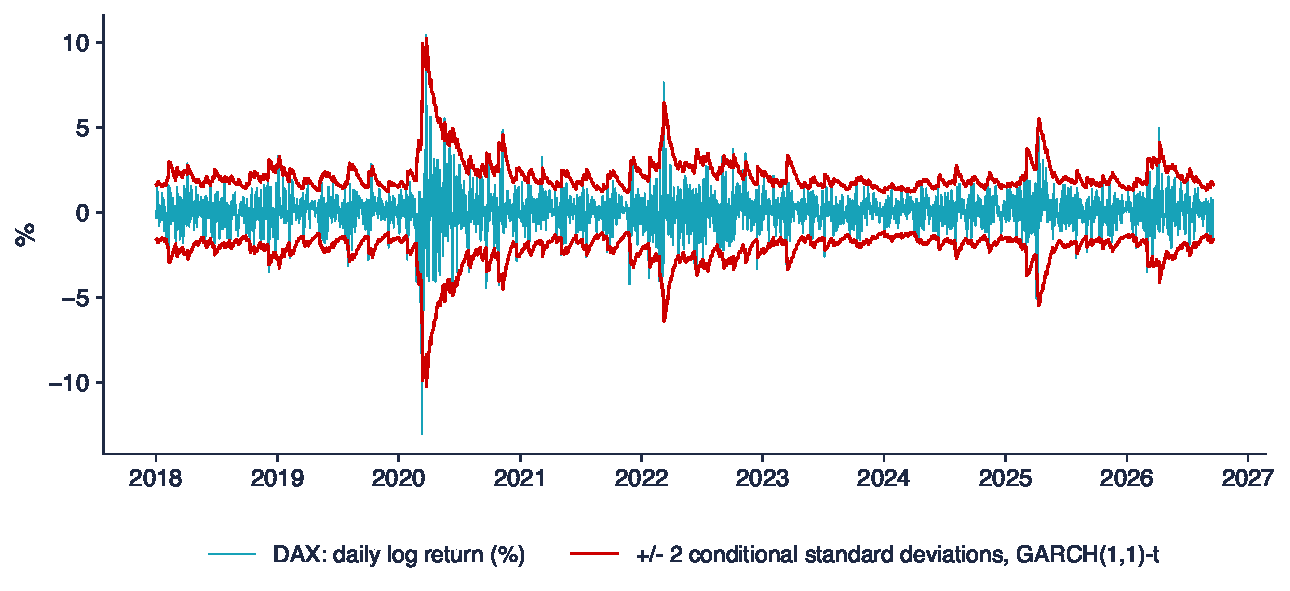
\includegraphics[width=0.96\textwidth,height=0.30\textheight,keepaspectratio]{ch9_sem_b1.pdf}
\end{center}
\vspace{-2mm}
\begin{center}
\scriptsize
\begin{tabular}{lrrrrr}
\toprule
& $\mu$ & $\omega$ & $\alpha$ & $\beta$ & $\nu$ \\
\midrule
estimare & $0{,}081$ & $0{,}0206$ & $0{,}097$ & $0{,}895$ & $7{,}08$ \\
SE robustă & $0{,}012$ & $0{,}0049$ & $0{,}011$ & $0{,}012$ & $0{,}62$ \\
\bottomrule
\end{tabular}
\end{center}
\begin{itemize}
    \item $T = 6\,786$; $\alpha + \beta = 0{,}992$, timpul de înjumătățire $\ln 0{,}5/(-0{,}00784) = 88{,}5$ zile; volatilitatea de lungă durată 25{,}9\%, față de 22{,}4\% în eșantion
    \item Vîrfuri: 80\% (2008), 82\% (2020); ultima zi: 13{,}0\%; 5{,}2\% dintre zile ies din banda $\pm 2\hat\sigma_t$
    \item Interpretare: pe cea curentă: VaR pentru mîine are nevoie de $\sigma_{t+1}$; nivelul de lungă durată contează doar pentru orizonturi lungi și este imprecis, deoarece $1 - \alpha - \beta = 0{,}0078$ este mic
\end{itemize}\sfmquantlet{Ch_09}{SFM_ch9_seminar}
\end{frame}

\begin{frame}{B2: BET, Banca Transilvania și Bitcoin [Propus]}
\itemsize{\footnotesize}
\begin{itemize}
\item \textbf{Întrebarea}: care dintre BET, Banca Transilvania și Bitcoin are volatilitatea cea mai persistentă? Model: B1.
\item \textbf{Date}: BET din 2000, TLV din 2010 (fără 30--31 mai 2016), Bitcoin din 2014; randamente logaritmice zilnice în \%
\item \textbf{Cerințe}
\begin{enumerate}
    \item Estimați GARCH(1,1)-t pentru fiecare serie și raportați $\alpha$, $\beta$ și $\nu$.
    \item Calculați persistența, timpul de înjumătățire și volatilitatea de lungă durată, acolo unde există.
    \item Comparați volatilitatea de lungă durată cu volatilitatea de selecție (anualizați Bitcoin cu 365 de zile).
    \item Interpretare: ce îi spune unui manager de risc o estimare $\hat\alpha + \hat\beta = 1$?
\end{enumerate}
\item \textbf{Raportați}: un tabel și două fraze
\item Notebook: secțiunea B2
\end{itemize}
\end{frame}

\ifsolutions
\begin{frame}{B2: rezolvare [Propus]}
\itemsize{\footnotesize}
\begin{center}
\scriptsize
\begin{tabular}{lrrrrrrrrr}
\toprule
& $T$ & $\alpha$ & $\beta$ & $\nu$ & $\alpha + \beta$ & înjumătățire & vol. lungă durată & vol. selecție & vîrf 2020 \\
\midrule
BET & 6\,670 & $0{,}192$ & $0{,}799$ & $5{,}01$ & $0{,}991$ & 74{,}3 & 34{,}7 & 22{,}1 & 88 \\
TLV & 3\,788 & $0{,}139$ & $0{,}824$ & $4{,}91$ & $0{,}963$ & 18{,}4 & 28{,}2 & 26{,}5 & 80 \\
Bitcoin & 4\,384 & $0{,}109$ & $0{,}891$ & $3{,}18$ & $1{,}000$ & -- & -- & 66{,}6 & 301 \\
\bottomrule
\end{tabular}
\end{center}
\begin{itemize}
    \item BET: cea mai puternică reacție ($\alpha = 0{,}192$) și un timp de înjumătățire de 74{,}3 zile; volatilitatea lui de lungă durată (34{,}7\%) este mult peste valoarea de selecție: un număr imprecis
    \item TLV: memorie mai scurtă (18{,}4 zile); volatilitatea de lungă durată și cea de selecție sînt apropiate (28{,}2\% și 26{,}5\%)
    \item Bitcoin: $\hat\alpha + \hat\beta = 1{,}0000$: un IGARCH, cel mai persistent; $\hat\nu = 3{,}18$
    \item Interpretare: nu există revenire la medie: prognozele pentru orice orizont sînt egale cu varianța de azi; modelul se comportă ca un EWMA, iar o volatilitate de lungă durată nu ar trebui raportată
\end{itemize}\sfmquantlet{Ch_09}{SFM_ch9_seminar}
\end{frame}
\fi

\begin{frame}{B3: efectul de levier la S\&P 500 [Rezolvat]}
\itemsize{\footnotesize}
\begin{itemize}
\item \textbf{Întrebarea}: cresc scăderile volatilitatea S\&P 500 mai mult decît creșterile de aceeași mărime?
\item \textbf{Date}: închiderile S\&P 500 din 2000, randamente logaritmice zilnice în \%
\item \textbf{Cerințe}
\begin{enumerate}
    \item Estimați GARCH(1,1)-t și GJR-GARCH(1,1)-t; raportați $\gamma$ cu statistica $t$ robustă.
    \item Calculați statistica LR pentru GJR față de GARCH, p-valoarea ei și cele două valori BIC.
    \item Aplicați testul de asimetrie (sign bias) pe reziduurile standardizate ale GARCH-t.
    \item Desenați ambele curbe de impact ale știrilor și calculați varianța GJR după șocuri de $-2\%$ și $+2\%$.
    \item Interpretare: cum schimbă efectul de levier VaR-ul din ziua de după o scădere?
\end{enumerate}
\item \textbf{Raportați}: patru statistici cu p-valori, două varianțe, graficul și două fraze
\item Notebook: secțiunea B3
\end{itemize}
\end{frame}

\begin{frame}{B3: rezolvare [Rezolvat]}
\itemsize{\scriptsize}
\begin{center}
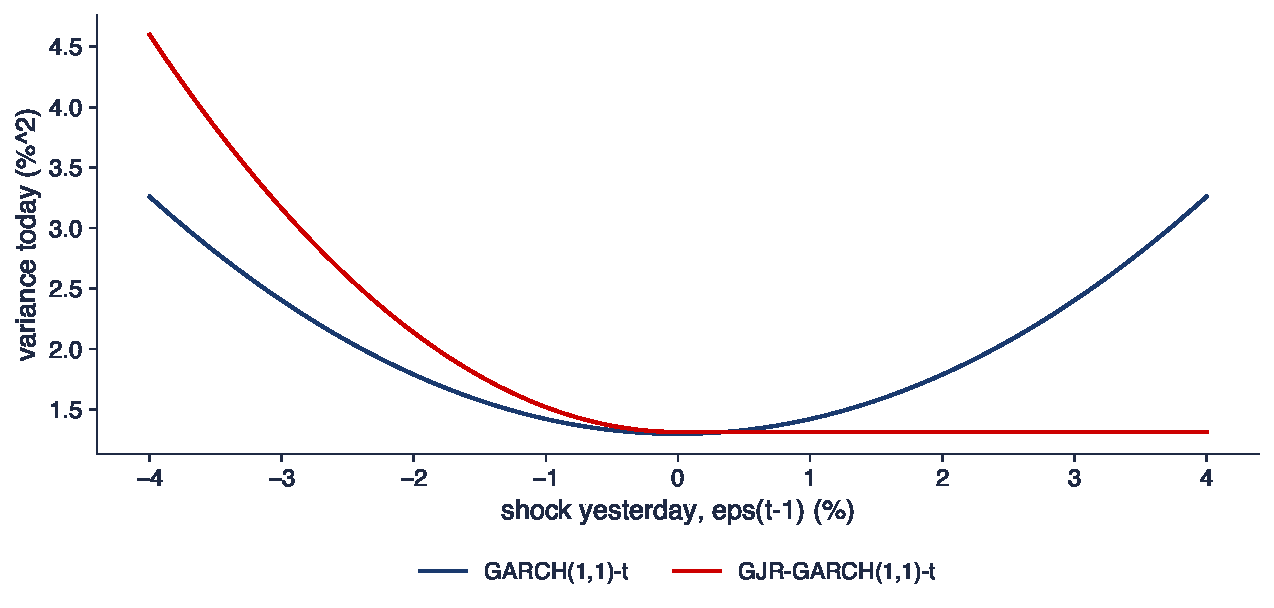
\includegraphics[width=0.96\textwidth,height=0.34\textheight,keepaspectratio]{ch9_sem_b3.pdf}
\end{center}
\vspace{-2mm}
\begin{itemize}
    \item GJR: $\hat\alpha = 0{,}000$, $\hat\gamma = 0{,}205$ ($t = 10{,}03$), $\hat\beta = 0{,}881$; LR $= 235{,}7$ (p $<$\,0{,}001); BIC $18169{,}0 \to 17942{,}2$
    \item Testul de asimetrie pe reziduurile GARCH-t: $\chi^2(3) = 40{,}7$ (p $<$\,0{,}001), $t$ al semnului $= 3{,}56$
    \item Varianța GJR după $-2\%$: $2{,}136$; după $+2\%$: $1{,}315$; raportul $1{,}62$
    \item Interpretare: doar scăderile cresc varianța ($\hat\alpha = 0$); după o scădere, VaR este de circa $\sqrt{1{,}62}$ ori VaR-ul de după o creștere egală; un GARCH simetric subestimează riscul după zilele proaste
\end{itemize}\sfmquantlet{Ch_09}{SFM_ch9_seminar}
\end{frame}

\begin{frame}{B4: asimetria la BVB și la Bitcoin [Propus]}
\itemsize{\footnotesize}
\begin{itemize}
\item \textbf{Întrebarea}: există un efect de levier la BET, la Banca Transilvania și la Bitcoin? Model: B3.
\item \textbf{Date}: BET din 2000, TLV din 2010, Bitcoin din 2014; randamente logaritmice zilnice în \%
\item \textbf{Cerințe}
\begin{enumerate}
    \item Estimați GJR-GARCH(1,1)-t și EGARCH(1,1)-t; raportați ambele valori $\gamma$, cu statisticile $t$ robuste.
    \item Calculați testul LR pentru GJR față de GARCH și modificarea BIC.
    \item Calculați raportul GJR dintre varianțele de după $-2\%$ și $+2\%$.
    \item Interpretare: ați folosi un model asimetric pentru fiecare dintre cele trei serii? De ce?
\end{enumerate}
\item \textbf{Raportați}: un tabel și două fraze
\item Notebook: secțiunea B4
\end{itemize}
\end{frame}

\ifsolutions
\begin{frame}{B4: rezolvare [Propus]}
\itemsize{\footnotesize}
\begin{center}
\footnotesize
\begin{tabular}{lrrrrrrrr}
\toprule
& GJR $\gamma$ & $t$ & LR & p & $\Delta$BIC & EGARCH $\gamma$ & $t$ & raport $-2/+2$ \\
\midrule
BET & $0{,}043$ & ${2{,}05}$ & $4{,}9$ & 0{,}026 & ${3{,}9}$ & ${-0{,}028}$ & ${-2{,}63}$ & $1{,}08$ \\
TLV & $0{,}065$ & ${2{,}71}$ & $7{,}8$ & 0{,}005 & ${0{,}4}$ & ${-0{,}040}$ & ${-3{,}00}$ & $1{,}08$ \\
Bitcoin & $-0{,}013$ & ${-0{,}72}$ & $0{,}7$ & 0{,}416 & ${7{,}7}$ & ${0{,}015}$ & ${1{,}18}$ & $1{,}00$ \\
\bottomrule
\end{tabular}
\end{center}
\begin{itemize}
    \item BET și TLV: $\gamma > 0$ (în EGARCH $\gamma < 0$), semnificativ după testul LR la 5\%, dar BIC crește ($\Delta$BIC $> 0$), iar raportul este doar 1{,}08 și, respectiv, 1{,}08
    \item Bitcoin: nicio asimetrie ($t = -0{,}72$; raportul 1{,}00)
    \item Interpretare: la BVB efectul este real, dar mic: GARCH-t este suficient pentru majoritatea aplicațiilor; pentru Bitcoin un model simetric este potrivit; pentru S\&P 500 (B3) asimetria este esențială
\end{itemize}\sfmquantlet{Ch_09}{SFM_ch9_seminar}
\end{frame}
\fi

\begin{frame}{B5: GARCH față de EWMA pentru S\&P 500 [Rezolvat]}
\itemsize{\footnotesize}
\begin{itemize}
\item \textbf{Întrebarea}: prognozează GARCH(1,1)-t varianța de mîine a S\&P 500 mai bine decît EWMA și este VaR 1\% al lui depășit în 1\% dintre zile?
\item \textbf{Date}: S\&P 500 din 2000; prognoze pentru fiecare zi de la 2 ianuarie 2015
\item \textbf{Cerințe}
\begin{enumerate}
    \item Reestimați GARCH(1,1)-t la fiecare 250 de zile pe toate datele pînă în acea zi și calculați prognozele pe o zi $h_t$; calculați EWMA cu $\lambda = 0{,}94$.
    \item Calculați media QLIKE pentru ambele modele și statistica $t$ Diebold--Mariano.
    \item Numărați depășirile VaR 1\% GARCH-t și VaR 1\% EWMA-Normal și comparați-le cu numărul așteptat.
    \item Desenați diferența cumulată a pierderilor.
    \item Interpretare: ce model i-ați da unui manager de risc și ce ați mai corecta?
\end{enumerate}
\item \textbf{Raportați}: patru valori, două numărători, graficul și două fraze
\item Notebook: secțiunea B5
\end{itemize}
\end{frame}

\begin{frame}{B5: rezolvare [Rezolvat]}
\itemsize{\scriptsize}
\begin{center}
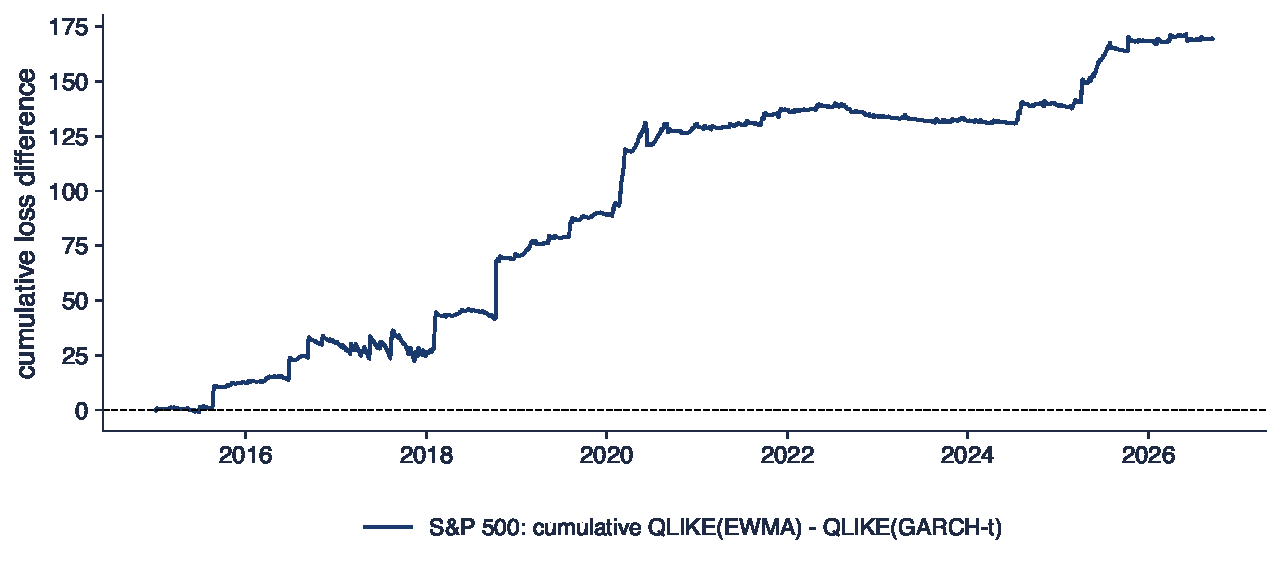
\includegraphics[width=0.96\textwidth,height=0.32\textheight,keepaspectratio]{ch9_sem_b5.pdf}
\end{center}
\vspace{-2mm}
\begin{itemize}
    \item 2\,944 de zile; media QLIKE: GARCH-t $0{,}761$, EWMA $0{,}819$; DM: diferența medie $-0{,}058$, $t = -3{,}69$ (p $<$\,0{,}001): GARCH-t este mai bun
    \item Depășiri VaR 1\%: GARCH-t 49 (1{,}66\%), EWMA-Normal 65 (2{,}21\%); așteptat circa 29
    \item Interpretare: GARCH-t, dar ambele modele VaR sînt depășite prea des; adăugăm efectul de levier (B3) și testăm formal depășirile (\sfmchlink{https://danpele.github.io/SFM/RO/Cursuri/capitol10_var_es_backtesting.pdf}{Capitolul 10})
\end{itemize}\sfmquantlet{Ch_09}{SFM_ch9_seminar}
\end{frame}

\begin{frame}{B6: GARCH față de EWMA pentru DAX și BET [Propus]}
\itemsize{\footnotesize}
\begin{itemize}
\item \textbf{Întrebarea}: se păstrează rezultatul din B5 pentru DAX și pentru BET? Model: B5.
\item \textbf{Date}: DAX și BET din 2000; prognoze pentru fiecare zi din ianuarie 2015
\item \textbf{Cerințe}
\begin{enumerate}
    \item Calculați prognozele GARCH(1,1)-t și EWMA în afara eșantionului, ca în B5.
    \item Calculați media QLIKE pentru ambele modele și testul DM.
    \item Numărați depășirile VaR 1\% pentru ambele modele.
    \item Interpretare: pentru care indice ajută cel mai mult GARCH și de ce?
\end{enumerate}
\item \textbf{Raportați}: un tabel și două fraze
\item Notebook: secțiunea B6
\end{itemize}
\end{frame}

\ifsolutions
\begin{frame}{B6: rezolvare [Propus]}
\itemsize{\footnotesize}
\begin{center}
\scriptsize
\begin{tabular}{lrrrrrrr}
\toprule
& zile & QLIKE GARCH-t & QLIKE EWMA & DM $t$ (p) & așteptat & dep. GARCH-t & dep. EWMA \\
\midrule
DAX & 2\,973 & $1{,}090$ & $1{,}121$ & ${-3{,}19}$ (0{,}001) & 30 & 45 (1{,}51\%) & 74 (2{,}49\%) \\
BET & 2\,926 & $0{,}680$ & $0{,}788$ & ${-2{,}22}$ (0{,}027) & 29 & 34 (1{,}16\%) & 67 (2{,}29\%) \\
\bottomrule
\end{tabular}
\end{center}
\begin{itemize}
    \item Ambii indici: GARCH-t are QLIKE mai mic, semnificativ la 5\% după testul DM
    \item BET: cel mai mare cîștig QLIKE și un VaR aproape exact (1{,}16\% față de 1\%); EWMA-Normal este depășit de circa două ori mai des decît ar trebui
    \item Interpretare: BET are cozi groase ($\nu \approx 5$) și salturi bruște ale volatilității: ajută atît cuantila Student-t, cît și revenirea la medie din GARCH
\end{itemize}\sfmquantlet{Ch_09}{SFM_ch9_seminar}
\end{frame}
\fi


%=============================================================================
\section{Partea C: întrebări deschise și critica unui răspuns AI}
%=============================================================================

\begin{frame}{C1: devine volatilitatea Bitcoin asemănătoare cu cea a acțiunilor? [Propus]}
\itemsize{\footnotesize}
\begin{itemize}
\item \textbf{Întrebarea}: s-a apropiat volatilitatea Bitcoin de volatilitatea S\&P 500 după 2021?
\item \textbf{Date}: randamentele logaritmice zilnice Bitcoin și S\&P 500, 2015--2019 și 2021--2026; modele: B1, B3
\item \textbf{Cerințe}
\begin{enumerate}
    \item Estimați GJR-GARCH(1,1)-t pentru ambele serii, în ambele perioade, și raportați persistența, $\gamma$ și $\nu$.
    \item Calculați corelația logaritmilor celor două volatilități GARCH-t în zilele comune, în fiecare perioadă.
    \item Enumerați evenimentele din 2020--2024 care ar putea explica o schimbare.
    \item Interpretare: cum ați deosebi o schimbare durabilă de o schimbare produsă de o singură criză?
\end{enumerate}
\item \textbf{Raportați}: un tabel și un plan de proiect
\item Notebook: secțiunea C1
\end{itemize}
\end{frame}

\ifsolutions
\begin{frame}{C1: analiză de referință [Propus]}
\itemsize{\footnotesize}
\begin{center}
\scriptsize
\begin{tabular}{lrrrrrr}
\toprule
Perioada & BTC $\alpha + \beta + \gamma/2$ & BTC $\gamma$ ($t$) & BTC $\nu$ & persistență S\&P & S\&P $\gamma$ ($t$) & corel.\ log-vol. \\
\midrule
2015--2019 & 1{,}000 & $-0{,}059$ ($-2{,}5$) & $3{,}23$ & $0{,}968$ & $0{,}344$ ($5{,}0$) & $0{,}04$ \\
2021--2026 & 1{,}000 & $0{,}037$ ($1{,}4$) & $3{,}28$ & $0{,}971$ & $0{,}196$ ($4{,}1$) & $0{,}32$ \\
\bottomrule
\end{tabular}
\end{center}
\begin{itemize}
    \item Bitcoin 2015--2019: $\gamma = -0{,}059$ ($t = -2{,}5$): creșterile au mărit volatilitatea mai mult decît scăderile (un efect de levier invers); 2021--2026: $\gamma = 0{,}037$ ($t = 1{,}4$), nesemnificativ
    \item Corelația celor două volatilități: de la $0{,}04$ la $0{,}32$; volatilitatea de selecție a Bitcoin: de la 74{,}3\% la 57{,}1\%; tot de tip IGARCH
    \item Evenimente: pandemia COVID-19 (2020), cumpărările instituționale (2021), prăbușirea pieței cripto din 2022, ETF-urile spot pe Bitcoin (2024); abordare: ferestre mobile, Ethereum și aurul ca termeni de comparație, un test al schimbării corelației
\end{itemize}\sfmquantlet{Ch_09}{SFM_ch9_seminar}
\end{frame}
\fi

\begin{frame}{C2: verificați un răspuns AI [Propus]}
\itemsize{\scriptsize}
\begin{itemize}
    \item Un student a cerut unui asistent AI să interpreteze un GARCH(1,1)-t estimat pentru S\&P 500 (date zilnice, din 2000): $\hat\omega = 0{,}0157$, $\hat\alpha = 0{,}123$, $\hat\beta = 0{,}872$, $\hat\nu = 6{,}26$. Răspunsul:
    \item \aiprompt{(a) alpha + beta = 0{,}995, deci un șoc de volatilitate dispare în aproximativ o săptămînă.}
    \item \aiprompt{(b) Varianța de lungă durată este omega/(1 - alpha) = 0{,}018, o volatilitate anuală de 2{,}1\%.}
    \item \aiprompt{(c) Un GJR estimat dă gamma = 0{,}205 > 0: știrile bune cresc volatilitatea mai mult decît știrile proaste.}
    \item \aiprompt{(d) Ljung-Box Q(10) al pătratelor reziduurilor standardizate = 13{,}6, p = 0{,}19: modelul GARCH-t este corect.}
    \item \aiprompt{(e) Cu inovații Student-t, VaR 1\% pe o zi este de 2,326 ori sigma(t+1).}
    \item \aiprompt{(f) EWMA cu lambda = 0,94 este un GARCH(1,1) cu omega = 0, alpha = 0,06, beta = 0,94.}
    \item Cerințe
    \begin{itemize}
        \item 1. Pentru fiecare afirmație, precizați dacă este corectă; dacă nu este, formulați afirmația corectă și, acolo unde se poate, dați valoarea corectă din notebook (secțiunea C2).
        \item 2. Raportați: o listă de șase verdicte, fiecare cu un rînd de justificare.
    \end{itemize}
\end{itemize}
\end{frame}

\ifsolutions
\begin{frame}{C2: rezolvare [Propus]}
\itemsize{\footnotesize}
\begin{itemize}
    \item (a) Greșit: timpul de înjumătățire este $\ln 0{,}5/\ln 0{,}995 = 131$ zile, circa jumătate de an
    \item (b) Greșit: $\bar\sigma^2 = \omega/(1 - \alpha - \beta) = 2{,}97$, o volatilitate de lungă durată de 27{,}3\% (imprecisă, deoarece $1 - \alpha - \beta$ este mic)
    \item (c) Greșit: $\gamma > 0$ se adaugă la panta șocurilor \textbf{negative}: știrile proaste cresc volatilitatea mai mult (efectul de levier)
    \item (d) Greșit: nu a rămas niciun efect ARCH, dar asta nu dovedește că modelul este corect; testul de asimetrie respinge ($\chi^2(3) = 40{,}7$): lipsește asimetria
    \item (e) Greșit: 2,326 este cuantila Normală; pentru $t$ standardizată cu $\nu = 6{,}26$ factorul este $2{,}557$
    \item (f) Corect: EWMA este un IGARCH fără constantă
\end{itemize}\sfmquantlet{Ch_09}{SFM_ch9_seminar}
\end{frame}
\fi


%=============================================================================
\section{Încheiere}
%=============================================================================

\begin{frame}{Idei de reținut}
\itemsize{\small}
\begin{itemize}
    \item $\alpha + \beta$ decide tot ce ține de termenul lung: timpul de înjumătățire, varianța de lungă durată, forma prognozelor
    \item Riscul pe mai multe zile este suma prognozelor zilnice ale varianței, nu $\sqrt{H}$ ori volatilitatea de azi
    \item Inovațiile cu cozi groase schimbă cuantila VaR; asimetria schimbă VaR-ul după zilele proaste
    \item Comparăm prognozele în afara eșantionului (QLIKE, DM), nu doar în eșantion (AIC, BIC)
    \item Un răspuns AI este o ciornă: verificați formula varianței de lungă durată, semnul lui $\gamma$ și cuantila
\end{itemize}
\end{frame}

\begin{frame}{După seminar}
\itemsize{\small}
\begin{itemize}
    \item Cursul 9 dezvoltă fiecare temă de azi: ARCH și GARCH, estimarea, inovațiile, asimetria, diagnosticul, prognozele, VaR
    \item Încercați cerințele [Propus] în notebook; rezolvările se discută la seminar
    \item C1 poate deveni un proiect de echipă: ferestre mobile, Ethereum și aurul ca termeni de comparație
    \item Lectură: \refFHH, cap.~13; exerciții în \refBHL, cap.~13; \refTsay, cap.~3
\end{itemize}
\end{frame}


%=============================================================================
\section{Bibliografie}
%=============================================================================

\begin{frame}{Bibliografie}
\itemsize{\tiny}
\begin{itemize}
    \item Bollerslev, T. (1986). \href{https://doi.org/10.1016/0304-4076(86)90063-1}{Generalized autoregressive conditional heteroskedasticity}. \textit{Journal of Econometrics}, 31(3), 307--327.
    \item Bollerslev, T. (1987). \href{https://doi.org/10.2307/1925546}{A conditionally heteroskedastic time series model for speculative prices and rates of return}. \textit{Review of Economics and Statistics}, 69(3), 542--547.
    \item Bollerslev, T., Wooldridge, J.M. (1992). \href{https://doi.org/10.1080/07474939208800229}{Quasi-maximum likelihood estimation and inference in dynamic models with time-varying covariances}. \textit{Econometric Reviews}, 11(2), 143--172.
    \item Borak, S., Härdle, W.K., López-Cabrera, B. (2013). \href{https://doi.org/10.1007/978-3-642-33929-5}{\textit{Statistics of Financial Markets: Exercises and Solutions}}, 2nd ed. Springer.
    \item Christie, A.A. (1982). \href{https://doi.org/10.1016/0304-405X(82)90018-6}{The stochastic behavior of common stock variances: value, leverage and interest rate effects}. \textit{Journal of Financial Economics}, 10(4), 407--432.
    \item Diebold, F.X., Mariano, R.S. (1995). \href{https://doi.org/10.1080/07350015.1995.10524599}{Comparing predictive accuracy}. \textit{Journal of Business \& Economic Statistics}, 13(3), 253--263.
    \item Engle, R.F. (1982). \href{https://doi.org/10.2307/1912773}{Autoregressive conditional heteroscedasticity with estimates of the variance of United Kingdom inflation}. \textit{Econometrica}, 50(4), 987--1007.
    \item Engle, R.F., Ng, V.K. (1993). \href{https://doi.org/10.1111/j.1540-6261.1993.tb05127.x}{Measuring and testing the impact of news on volatility}. \textit{Journal of Finance}, 48(5), 1749--1778.
    \item Franke, J., Härdle, W.K., Hafner, C.M. (2019). \href{https://doi.org/10.1007/978-3-030-13751-9}{\textit{Statistics of Financial Markets: An Introduction}}, 5th ed. Springer.
    \item Glosten, L.R., Jagannathan, R., Runkle, D.E. (1993). \href{https://doi.org/10.1111/j.1540-6261.1993.tb05128.x}{On the relation between the expected value and the volatility of the nominal excess return on stocks}. \textit{Journal of Finance}, 48(5), 1779--1801.
    \item Hansen, B.E. (1994). \href{https://doi.org/10.2307/2527081}{Autoregressive conditional density estimation}. \textit{International Economic Review}, 35(3), 705--730.
    \item Ljung, G.M., Box, G.E.P. (1978). \href{https://doi.org/10.1093/biomet/65.2.297}{On a measure of lack of fit in time series models}. \textit{Biometrika}, 65(2), 297--303.
    \item Nelson, D.B. (1991). \href{https://doi.org/10.2307/2938260}{Conditional heteroskedasticity in asset returns: a new approach}. \textit{Econometrica}, 59(2), 347--370.
    \item Patton, A.J. (2011). \href{https://doi.org/10.1016/j.jeconom.2010.03.034}{Volatility forecast comparison using imperfect volatility proxies}. \textit{Journal of Econometrics}, 160(1), 246--256.
    \item Tsay, R.S. (2010). \href{https://doi.org/10.1002/9780470644560}{\textit{Analysis of Financial Time Series}}, 3rd ed. Wiley.
\end{itemize}
\end{frame}

\end{document}
